%\documentclass[smallcondensed]{svjour3} %一段組用
\documentclass[twocolumn]{svjour3}


\usepackage{enumitem}


\usepackage{color}

\usepackage{graphicx}
\usepackage{tikz}
\usepackage{calc}
\usepackage{array}

\usepackage{amsmath, amssymb}
\DeclareMathOperator*{\argmin}{arg\,min}

\usepackage{graphbox}
\usepackage{wasysym}

\usetikzlibrary{automata,arrows}

\usepackage{comment}

\usepackage{wrapfig}
\usepackage{hyperref}
\usepackage{supertabular}

\tikzstyle{mol} = [fill, circle, inner sep=1pt]




\begin{document}

\title{Counting infinitely by oritatami co-transcriptional folding\thanks{A version of this work with several details omitted was published in the proceedings of the 46th International Conference on Current Trends in Theory and Practice of Computer Science (SOFSEM 2020, Limassol, Cyprus, January 20-24, 2020), LNCS, 12011, pp. 566--575.}}

%\titlerunning{}
\author{
Kohei Maruyama\and
Shinnosuke Seki
}
\institute{
K. Maruyama \at
The University of Electro-Communications, 1-5-1 Chofugaoka, Chofu, Tokyo, 1828585, Japan\\
\email{k.maruyama@uec.ac.jp}
\and
S. Seki \at
The University of Electro-Communications, 1-5-1 Chofugaoka, Chofu, Tokyo, 1828585, Japan\\
\'{E}cole Normale Superi\'{e}ure de Lyon, 46 all\'{e}e d'Italie, 69007, Lyon, France\\
\email{s.seki@uec.ac.jp}
}

\date{Received: date / Accepted: date}
% The correct dates will be entered by the editor

\maketitle


\begin{abstract}
A fixed bit-width counter was proposed as a proof-of-concept demonstration of an oritatami model of cotranscriptional folding [Geary et al., Proc.~MFCS 2016, LIPIcs 58, 43:1-43:14], and it was embedded into another oritatami system that self-assembles a finite portion of Heighway dragon fractal. 
In order to expand its applications, we endow this counter with capability to widen bit-width at every encounter with overflow. 
\end{abstract}

%------------------------------------------------------
	\section{Introduction}
%------------------------------------------------------

Counting is one of the most essential tasks for computing; as well known, the ability to count suffices to enable Turing universality \cite{Minsky1967}. 
Nature has been counting billions of days using molecular ``circadian clockwork'' which is ``as complicated and as beautiful as the wonderful chronometers developed in the 18th century''  \cite{McClung2006}. 
Nowadays, developments in molecular self-assembly technology enable us to design molecules to count. 
Evans has demonstrated a DNA tile self-assembly system that counts accurately \textit{in-vitro} in binary from a programmed initial count until it overflows \cite{EvansPhD}. 
In its foundational theory of molecular self-assembly, such binary counters have been proved versatile, being used to assemble shapes of particular size \cite{AdChGoHu2001,RothemundWinfree2000}, towards self-assembly of fractals \cite{MasudaSekiUbukata2018}, as an infinite scaffold to simulate all Turing machines in parallel in order to prove undecidability of nondeterminism in the abstract tile-assembly model \cite{BrChDoKaSe2013}, to name a few. 

\begin{figure}[tb]
\centering
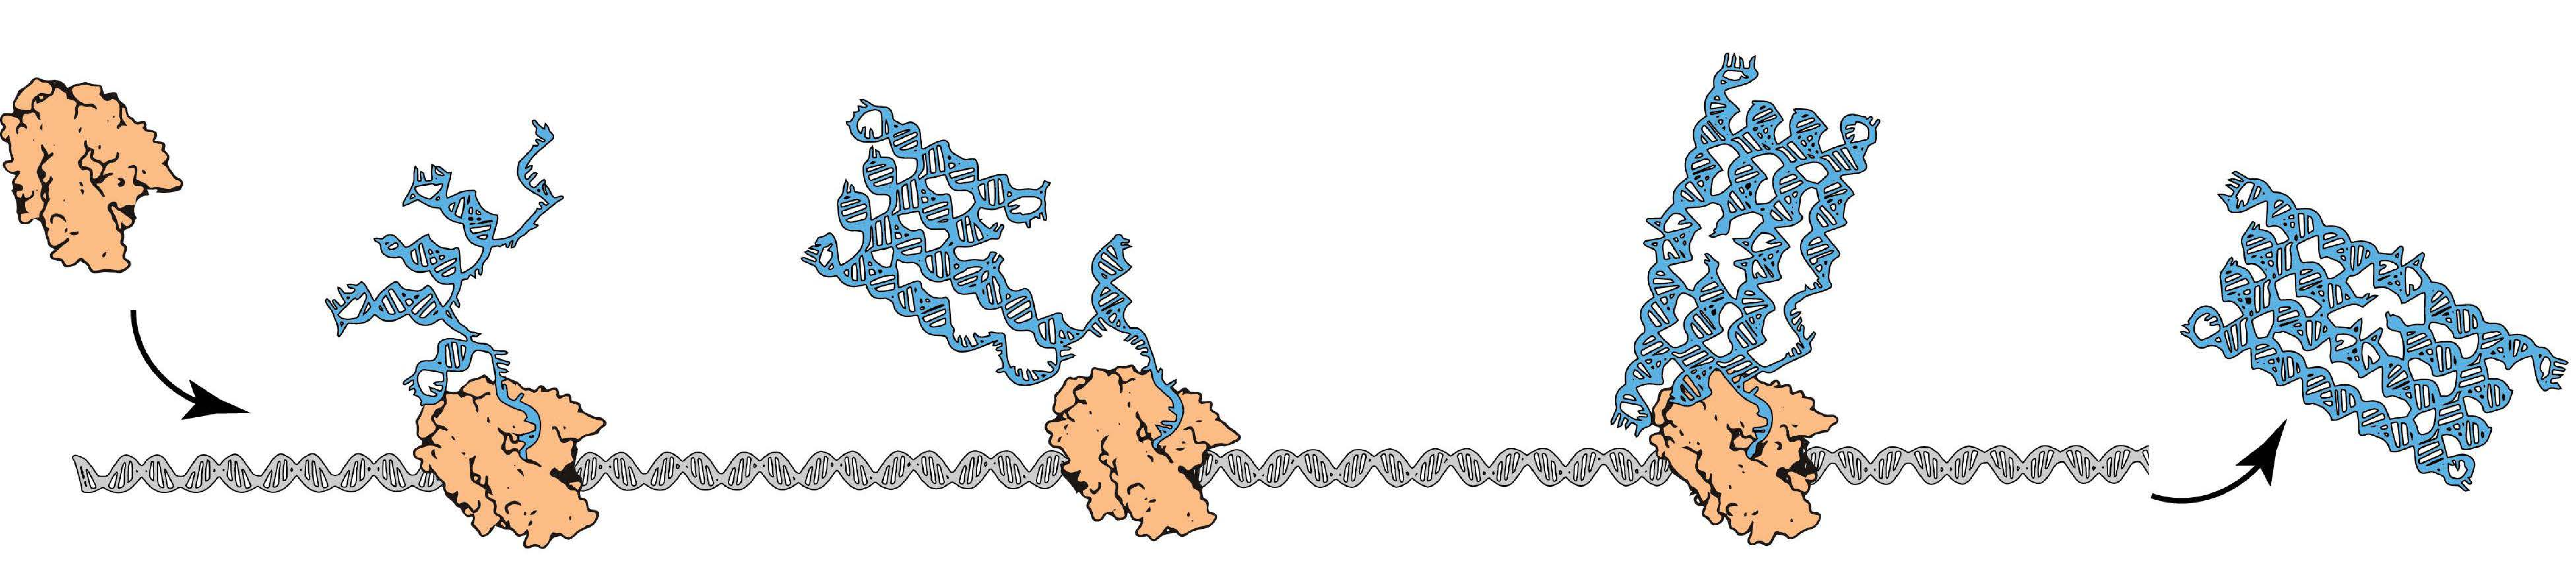
\includegraphics[width=\linewidth]{fig/rna_origami.pdf}
\caption{RNA origami. RNA polymerase enzyme (orange) synthesizes the temporal copy (blue) of a gene (gray spiral) out of ribonucleotides of four types A, C, G, and U.}
\label{fig:rna_origami}
\end{figure}

A fixed bit-width (finite) binary counter has been implemented as a proof-of-concept demonstration of the oritatami model of cotranscriptional folding \cite{GeMeScSe2019}. 
As shown in Fig.~\ref{fig:rna_origami}, an RNA transcript folds upon itself while being transcribed (synthesized) from its corresponding DNA template strand. 
Geary et al. programmed a specific RNA rectangular tile structure into a DNA template in such a way that the corresponding RNA transcript \textit{folds cotranscriptionally} into the programmed tile structure with high probability \textit{in vitro} at room temperatures (\textit{RNA origami}) \cite{GearyRothemundAndersen2014}. 
An oritatami system folds a transcript of abstract molecules called \textit{beads} of finitely many types over the 2-dimensional triangular lattice cotranscriptionally according to a rule set that specifies which types of molecules are allowed to bind once they are placed at the unit distance away. 
The transcript of the binary counter in \cite{GeMeScSe2019} is of period 60 as $\textcircled{\scriptsize 0}{-}\textcircled{\scriptsize 1}{-}\textcircled{\scriptsize 2}{-} \cdots {-}\textcircled{\scriptsize 58}{-}\textcircled{\scriptsize 59}{-}\textcircled{\scriptsize 0}{-}\textcircled{\scriptsize 1} \cdots$ and its period is semantically divided into two half-adder (HA) modules $A = \textcircled{\scriptsize 0}{-}\textcircled{\scriptsize 1}{-} \cdots {-}\textcircled{\scriptsize 11}$ and $C = \textcircled{\scriptsize 30}{-}\textcircled{\scriptsize 31}{-} \cdots {-}\textcircled{\scriptsize 41}$ and two structural modules $B$ and $D$, which are sandwiched by half-adder modules along the transcript.
While being folded cotranscriptionally in zigzags, HA modules increment the current count $i$ by 1, which is initialized on a linear \textit{seed} structure, alike the Evans' counter, whereas structural modules $B$ and $D$ align HA modules properly and also make a turn at an end of the count $i$; $B$ guides the transcript from a zig to a zag ($\hookrightarrow$) while $D$ does from a zag to a zig ($\hookleftarrow$). 
This counter was embedded as a component of an oritatami system to self-assemble an arbitrary finite portion of Heighway dragon fractal \cite{MasudaSekiUbukata2018}. 
Its applications are limited, however, by lack of mechanism to widen bit-width; its behavior is undefined when its count overflows. 
In this paper, we endow this counter, or more precisely, its structural module $B$, with the capability to widen the count by 1 bit at every encounter with overflow. 




%Our body consists many proteins which is based on genetic sequence in DNA.
%DNA sequence has to be copied in order to make proteins because DNA is in cell nucleus.
%It is copied to RNA (and its sequence is called \textit{transcript}) by a RNA polymerase and delivered to out of nucleus.
%A transcript consists four types nucleobases A, U, G, and C, and a nucleobase are called \textit{bead}
%Moreover, they form hydrogen bonds mainly between A and U, and between G and C, then they begin to form at the same time synthesizing.
%Once the bead is fixed after that it can not change the position.
%By repeating this method, transcript form a 3D shape.
%
%A shape of RNA depends on the DNA sequence.
%Geary, Rothemund, and Andrsen have succeeded in experimentally making 2D RNA tiles (Fig.\ref{fig:rna_origami}) by repeatedly copying a specific DNA sequence \cite{GearyRothemundAndersen2014}.
%Then, Oritatami System was designed as a mathematical model that the process of RNA production \cite{counter2016} and Fig.\ref{fig:origami_on_oritatami} is the 2D RNA tile which is represented on Oritatami System.
%Oritatami system treats transcript and nucleobase as paths and vertices which called \textit{bead}, respectively, moreover, they are arranged on a triangular grid.
%The system takes transcript as an input and output an terminal conformation.
%Geary et al. implemented binary counter in this system \cite{counter2016}.
%This counter is folded in zigzags, and each row represents a counted number.
%Then, this counter is given a bit width as an input to the system before transfer begins, and encounters nondeterminism if it carries beyond that bit width.
%Since it is running on deterministic system, it halts when it becomes nondeterministic.
%
%In this paper, based on the implementation method of this counter, we implement a counter which defined the behavior that extends the bit width when it overflows.



%\begin{figure}[tb]
%\centering
%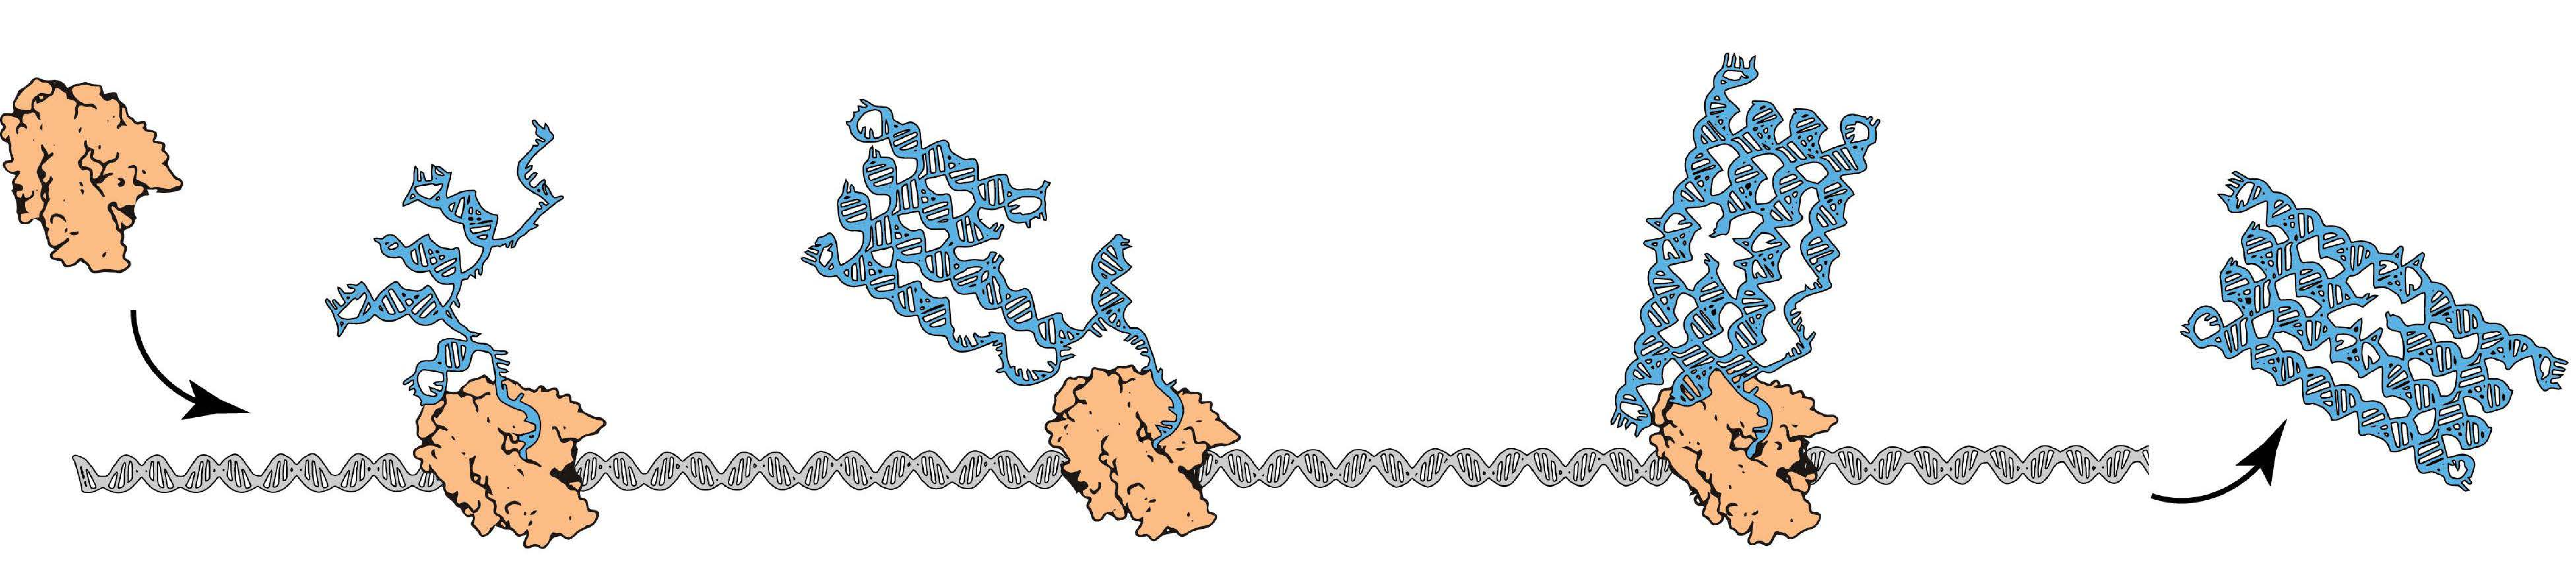
\includegraphics[width=\linewidth]{fig/rna_origami.pdf}
%\caption{
%A generated and stabilized 2D RNA tile from DNA
%}
%\label{fig:rna_origami}
%\end{figure}
%
%\begin{figure}[tb]
%\centering
%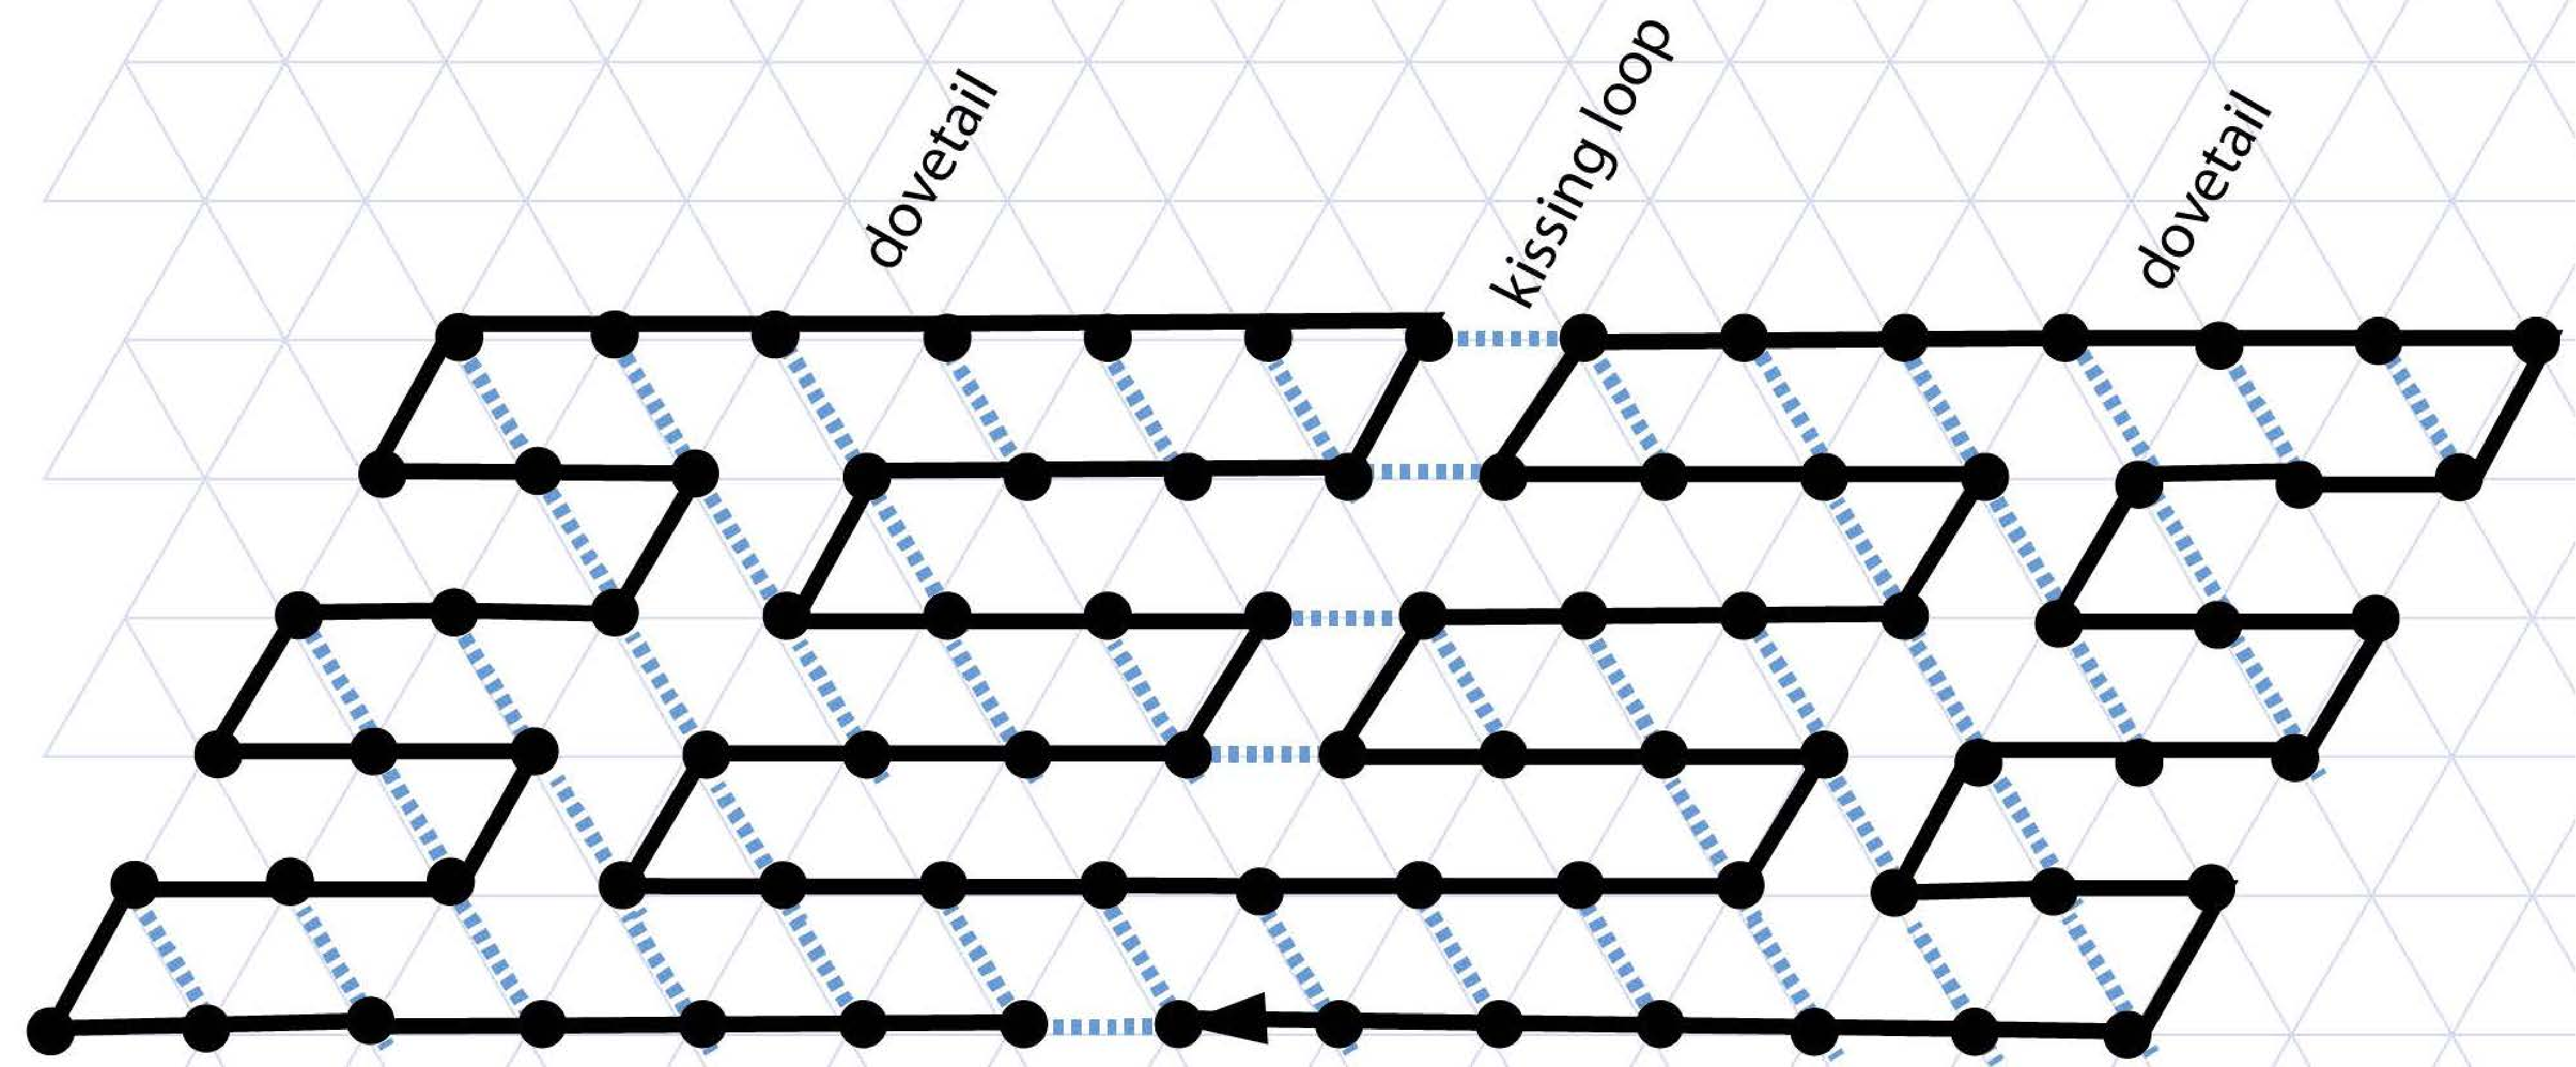
\includegraphics[width=\linewidth]{fig/origami_oritatami.pdf}
%\caption{
%The represented 2D RNA tile on Oritatami System
%}
%\label{fig:origami_on_oritatami}
%\end{figure}



%------------------------------------------------------
	\section{Preliminaries}
%------------------------------------------------------

%copy from TAMC2019 paper

Let $\Sigma$ be a finite alphabet, whose elements should be regarded as types of abstract molecule, or \textit{beads}. 
A bead of type $a \in \Sigma$ is called an $a$-bead. 
By $\Sigma^*$ and $\Sigma^\omega$, we denote the set of finite sequences of beads and that of one-way infinite sequences of beads, respectively. 
The empty sequence is denoted by $\lambda$. 
Let $w = b_1 b_2 \cdots b_n \in \Sigma^*$ be a sequence of length $n$ for some integer $n$ and bead types $b_1, \ldots, b_n \in \Sigma$. 
The \textit{length} of $w$ is denoted by $|w|$, that is, $|w| = n$. %ここから要らない?↓やっぱり要る
For two indices $i, j$ with $1 \le i \le j \le n$, we let $w[i..j]$ refer to the subsequence $b_i b_{i+1} \cdots b_{j-1}b_j$; if $i = j$, then $w[i..i]$ is simplified as $w[i]$. 
For $k \ge 1$, $w[1..k]$ is called a \textit{prefix} of $w$. 

Oritatami systems fold their transcript, which is a sequence of beads, over the triangular grid graph $\mathbb{T} = (V, E)$ cotranscriptionally. %↓
For a point $p \in V$, let $\hexagon_p^d$ denote the set of points which lie in the regular hexagon of radius $d$ centered at the point $p$. 
Note that $\hexagon_p^d$ consists of $3d(d+1)+1$ points. %←
A directed path $P = p_1 p_2 \cdots p_n$ in $\mathbb{T}$ is a sequence of \textit{pairwise-distinct} points $p_1, p_2, \ldots, p_n \in V$ such that $\{p_i, p_{i+1}\} \in E$ for all $1 \le i < n$. 
Its $i$-th point is referred to as $P[i]$. 
Now we are ready to abstract RNA single-stranded structures in the name of conformation. 
A \textit{conformation} $C$ (over $\Sigma$) is a triple $(P, w, H)$ of a directed path $P$ in $\mathbb{T}$, $w \in \Sigma^*$ of the same length as $P$, and a set of h-interactions $H \subseteq \bigl\{\{i, j\} \bigm| 1 \le i, i+2 \le j, \{P[i], P[j]\} \in E \bigr\}$. 
This is to be interpreted as the sequence $w$ being folded along the path $P$ in such a manner that its $i$-th bead $w[i]$ is placed at the $i$-th point $P[i]$ and the $i$-th and $j$-th beads are bound (by a hydrogen-bond-based interaction) if and only if $\{i, j\} \in H$. 
The condition $i+2 \le j$ represents the topological restriction that two consecutive beads along the path cannot be bound. 
The \textit{length} of $C$ is defined to be the length of its transcript $w$ (that is, equal to the length of the path $P$). 
A \textit{rule set} $R \subseteq \Sigma \times \Sigma$ is a symmetric relation over $\Sigma$, that is, for all bead types $a, b \in \Sigma$, $(a, b) \in R$ implies $(b, a) \in R$.
A bond $\{i, j\} \in H$ is \textit{valid with respect to $R$}, or simply $R$-valid, if $(w[i], w[j]) \in R$. 
This conformation $C$ is \textit{$R$-valid} if all of its bonds are $R$-valid. %↓
For an integer $\alpha \ge 1$, $C$ is \textit{of arity $\alpha$} if it contains a bead that forms $\alpha$ bonds but none of its beads forms more. 
By $\mathcal{C}_{\le \alpha}(\Sigma)$, we denote the set of all conformations over $\Sigma$ whose arity is at most $\alpha$; its argument $\Sigma$ is omitted whenever $\Sigma$ is clear from the context. 

The oritatami system grows conformations by an operation called elongation. 
Given a rule set $R$ and an $R$-valid conformation $C_1 = (P, w, H)$, we say that another conformation $C_2$ is an elongation of $C_1$ by a bead $b \in \Sigma$, written as $C_1 \xrightarrow{R}_b C_2$, if $C_2 = (P p, wb, H \cup H')$ for some point $p \in V$ not along the path $P$ and set $H' \subseteq \bigl\{ \{i, |w|+1\} \bigm| 1 \le i < |w|, \{P[i], p\} \in E, (w[i], b) \in R \bigr\}$ of bonds formed by the $b$-bead; this set $H'$ can be empty. 
Note that $C_2$ is also $R$-valid. 
This operation is recursively extended to the elongation by a finite sequence of beads as: for any conformation $C$, $C \xrightarrow{R}_\lambda^* C$; and for a finite sequence of beads $w \in \Sigma^*$ and a bead $b \in \Sigma$, a conformation $C_1$ is elongated to a conformation $C_2$ by $wb$, written as $C_1 \xrightarrow{R}_{wb}^* C_2$, if there is a conformation $C'$ that satisfies $C_1 \xrightarrow{R}_w^* C'$ and $C' \xrightarrow{R}_b C_2$. 

An \textit{oritatami system} (OS) $\Xi$ is a tuple $(\Sigma, R, \delta, \alpha, \sigma, w)$, where $\Sigma$ and $R$ are defined as above, while the other elements are
a positive integer $\delta$ called \textit{delay}, 
a positive integer $\alpha$ called \textit{arity},
an initial $R$-valid conformation $\sigma \in C_{\le \alpha}(\Sigma)$ called the \textit{seed},
and a (possibly infinite) \textit{transcript} $w \in \Sigma^* \cup \Sigma^\omega$, which is to be folded upon the seed by stabilizing beads of $w$ one at a time so as to minimize energy collaboratively with the succeeding $\delta{-}1$ nascent beads.
%
The energy of a conformation $C = (P, w, H)$, denoted by $\Delta G(C)$, is defined to be ${-}|H|$; the more bonds a conformation has, the more stable it gets. 
The set $\mathcal{F}(\Xi)$ of conformations \textit{foldable} by the system $\Xi$ is recursively defined as: the seed $\sigma$ is in $\mathcal{F}(\Xi)$; and provided that an elongation $C_i$ of $\sigma$ by the prefix $w[1..i]$ be foldable (i.e., $C_0 = \sigma$), its further elongation $C_{i+1}$ by the next bead $w[i+1]$ is foldable if 
\begin{equation}\label{eq:OS_CF}
C_{i+1} \in \argmin_{
\substack{
C \in \mathcal{C}_{\le \alpha} s.t. \\
C_i \xrightarrow{R}_{w[i+1]}C \\
}
}
\min \Bigl\{ \Delta G(C') \Bigm|
C \xrightarrow{R}^*_{w[i+2...i+k]}C', k\le \delta, C' \in \mathcal{C}_{\le \alpha}
\Bigr\}.
\end{equation}
%
Then we say that the bead $w[i+1]$ and the bonds it forms are \textit{stabilized} according to $C_{i+1}$. 
The easiest way to understand this stabilization process should be the video available at
\[
\mbox{\href{https://www.dailymotion.com/video/x3cdj35}{\texttt{https://www.dailymotion.com\slash video\slash x3cdj35}}}, 
\]
in which the Turing universal oritatami system by Geary et al. \cite{GeMeScSe2018}, whose delay is 3, is running.
This video is worth watching because a directed motif called a \textit{glider}, which it features, is utilized for our infinite counter.
Note that an arity-$\alpha$ oritatami system cannot fold any conformation of arity larger than $\alpha$. %←
A conformation foldable by $\Xi$ is \textit{terminal} if none of its elongations is foldable by $\Xi$. 
%The oritatami system $\Xi$ is \textit{deterministic} if for all $i \ge 0$, there exists at most one $C_{i+1}$ that satisfies \eqref{eq:OS_CF}. 
%A deterministic oritatami system folds into a unique terminal conformation. 
%An oritatami system with the empty rule set just folds into an arbitrary elongation of its seed nondeterministically. 
%Thus, the rule set is reasonably assumed non-empty. 

\begin{figure*}[tb]
\centering
\scalebox{0.8}{
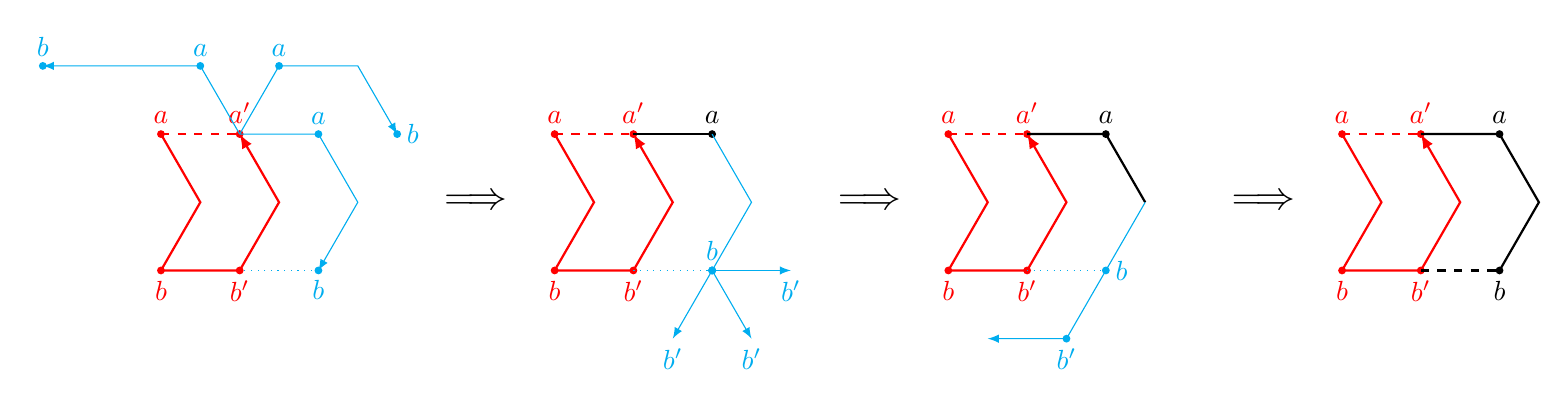
\begin{tikzpicture}

\foreach \x in {0, 5, 10, 15} {
\draw[red, thick, -latex] (\x, 0) node[mol] {} node[above] {$a$}
-- ++(300:1)
-- ++(240:1) node[mol] {} node[below] {$b$}
-- ++(0:1) node[mol] {} node[below] {$b'$}
-- ++(60:1)
-- ++(120:1) node[mol] {} node[above] {$a'$}
;
\draw[red, dashed, thick] (\x, 0) -- ++(0:1);
}

\draw[cyan, -latex] (1, 0) 
-- ++(120:1) node[mol] {} node[above] {$a$}
-- ++(180:2) node[mol] {} node[above] {$b$}
;
\draw[cyan, -latex] (1, 0) 
-- ++(60:1) node[mol] {} node[above] {$a$}
-- ++(0:1) 
-- ++(300:1) node[mol] {} node[right] {$b$}
;
\draw[cyan, -latex] (1, 0) 
-- ++(0:1) node[mol] {} node[above] {$a$}
-- ++(300:1) 
-- ++(240:1) node[mol] {} node[below] {$b$}
;
\draw[cyan, dotted] (1, 0)++(300:2) -- ++(180:1);

\draw (3.5, 0)++(300:1) node {\Large $\Longrightarrow$};

\draw[thick] (6, 0) -- ++(0:1) node[mol] {} node[above] {$a$};

\draw[cyan, -latex] (7, 0) 
-- ++(300:1) 
-- ++(240:1) node[mol] {} node[above] {$b$} 
-- ++(240:1) node[below] {$b'$}
; 
\draw[cyan, -latex] (7, 0) 
++(300:1) 
++(240:1) node[mol] {} node[above] {} 
-- ++(300:1) node[below] {$b'$}
; 
\draw[cyan, -latex] (7, 0) 
++(300:1) 
++(240:1) node[mol] {} node[above] {} 
-- ++(0:1) node[below] {$b'$}
; 
\draw[cyan, dotted] (5, 0)++(300:2) -- ++(0:1);

\draw (8.5, 0)++(300:1) node {\Large $\Longrightarrow$};

\draw[thick] (11, 0) -- ++(0:1) node[mol] {} node[above] {$a$} -- ++(300:1);

\draw[cyan, -latex] (12,0)++(300:1) -- ++(240:1) node[mol] {} node[right] {$b$} -- ++(240:1) node[mol] {} node[below] {$b'$} -- ++(180:1);

\draw[cyan, dotted] (10, 0)++(300:2) -- ++(0:1);

\draw (13.5, 0)++(300:1) node {\Large $\Longrightarrow$};

\draw[thick] (16, 0) -- ++(0:1) node[mol] {} node[above] {$a$} -- ++(300:1) -- ++(240:1) node[mol] {} node[below] {$b$};

\draw[thick,dashed] (15,0)++(300:2) -- ++(0:1);
\end{tikzpicture}}
\caption{Folding of a glider motif by a delay-3 deterministic oritatami system.}
\label{fig:glider}
\end{figure*}

\begin{example}[Glider\footnote{A video to show how a glider folds can be found at \href{https://www.dailymotion.com/video/x3cdj35}{\texttt{https://www.dailymotion.com/video/x3cdj35}}.}]
	See Fig.~\ref{fig:glider} for a delay-3 oritatami system $\Xi$ to fold a motif called a glider. 
	Its transcript is a repetition of $a \bullet b b' \bullet a$ and its rule set $R$ is $\{(a, a'), (b, b')\}$. 
	Its seed is colored in red. 
	The first 3 beads, $a \bullet b$, are transcribed and elongate the seed in all possible ways. 
	The $a$-bead cannot bind or the second bead is inert according to $R$. 
	The third bead, $b$, can bind to the $b'$-bead in the seed but for that, the $a$-bead must be located to the east of the previous $a'$-bead; it is thus stabilized there. 
	Then the next bead, $b'$, is transcribed. 
	After the three steps, the third bead, $b$, is stabilized. 
	It is not until then that its h-interaction with the $b'$-bead is also stabilized. 
\end{example}
%gliderが自立する構造であること


%%%%%%%%%%%
%%%%%%%%%%
%%%%%%%%%
%%%%%%%%

\begin{figure*}[p]
\centering
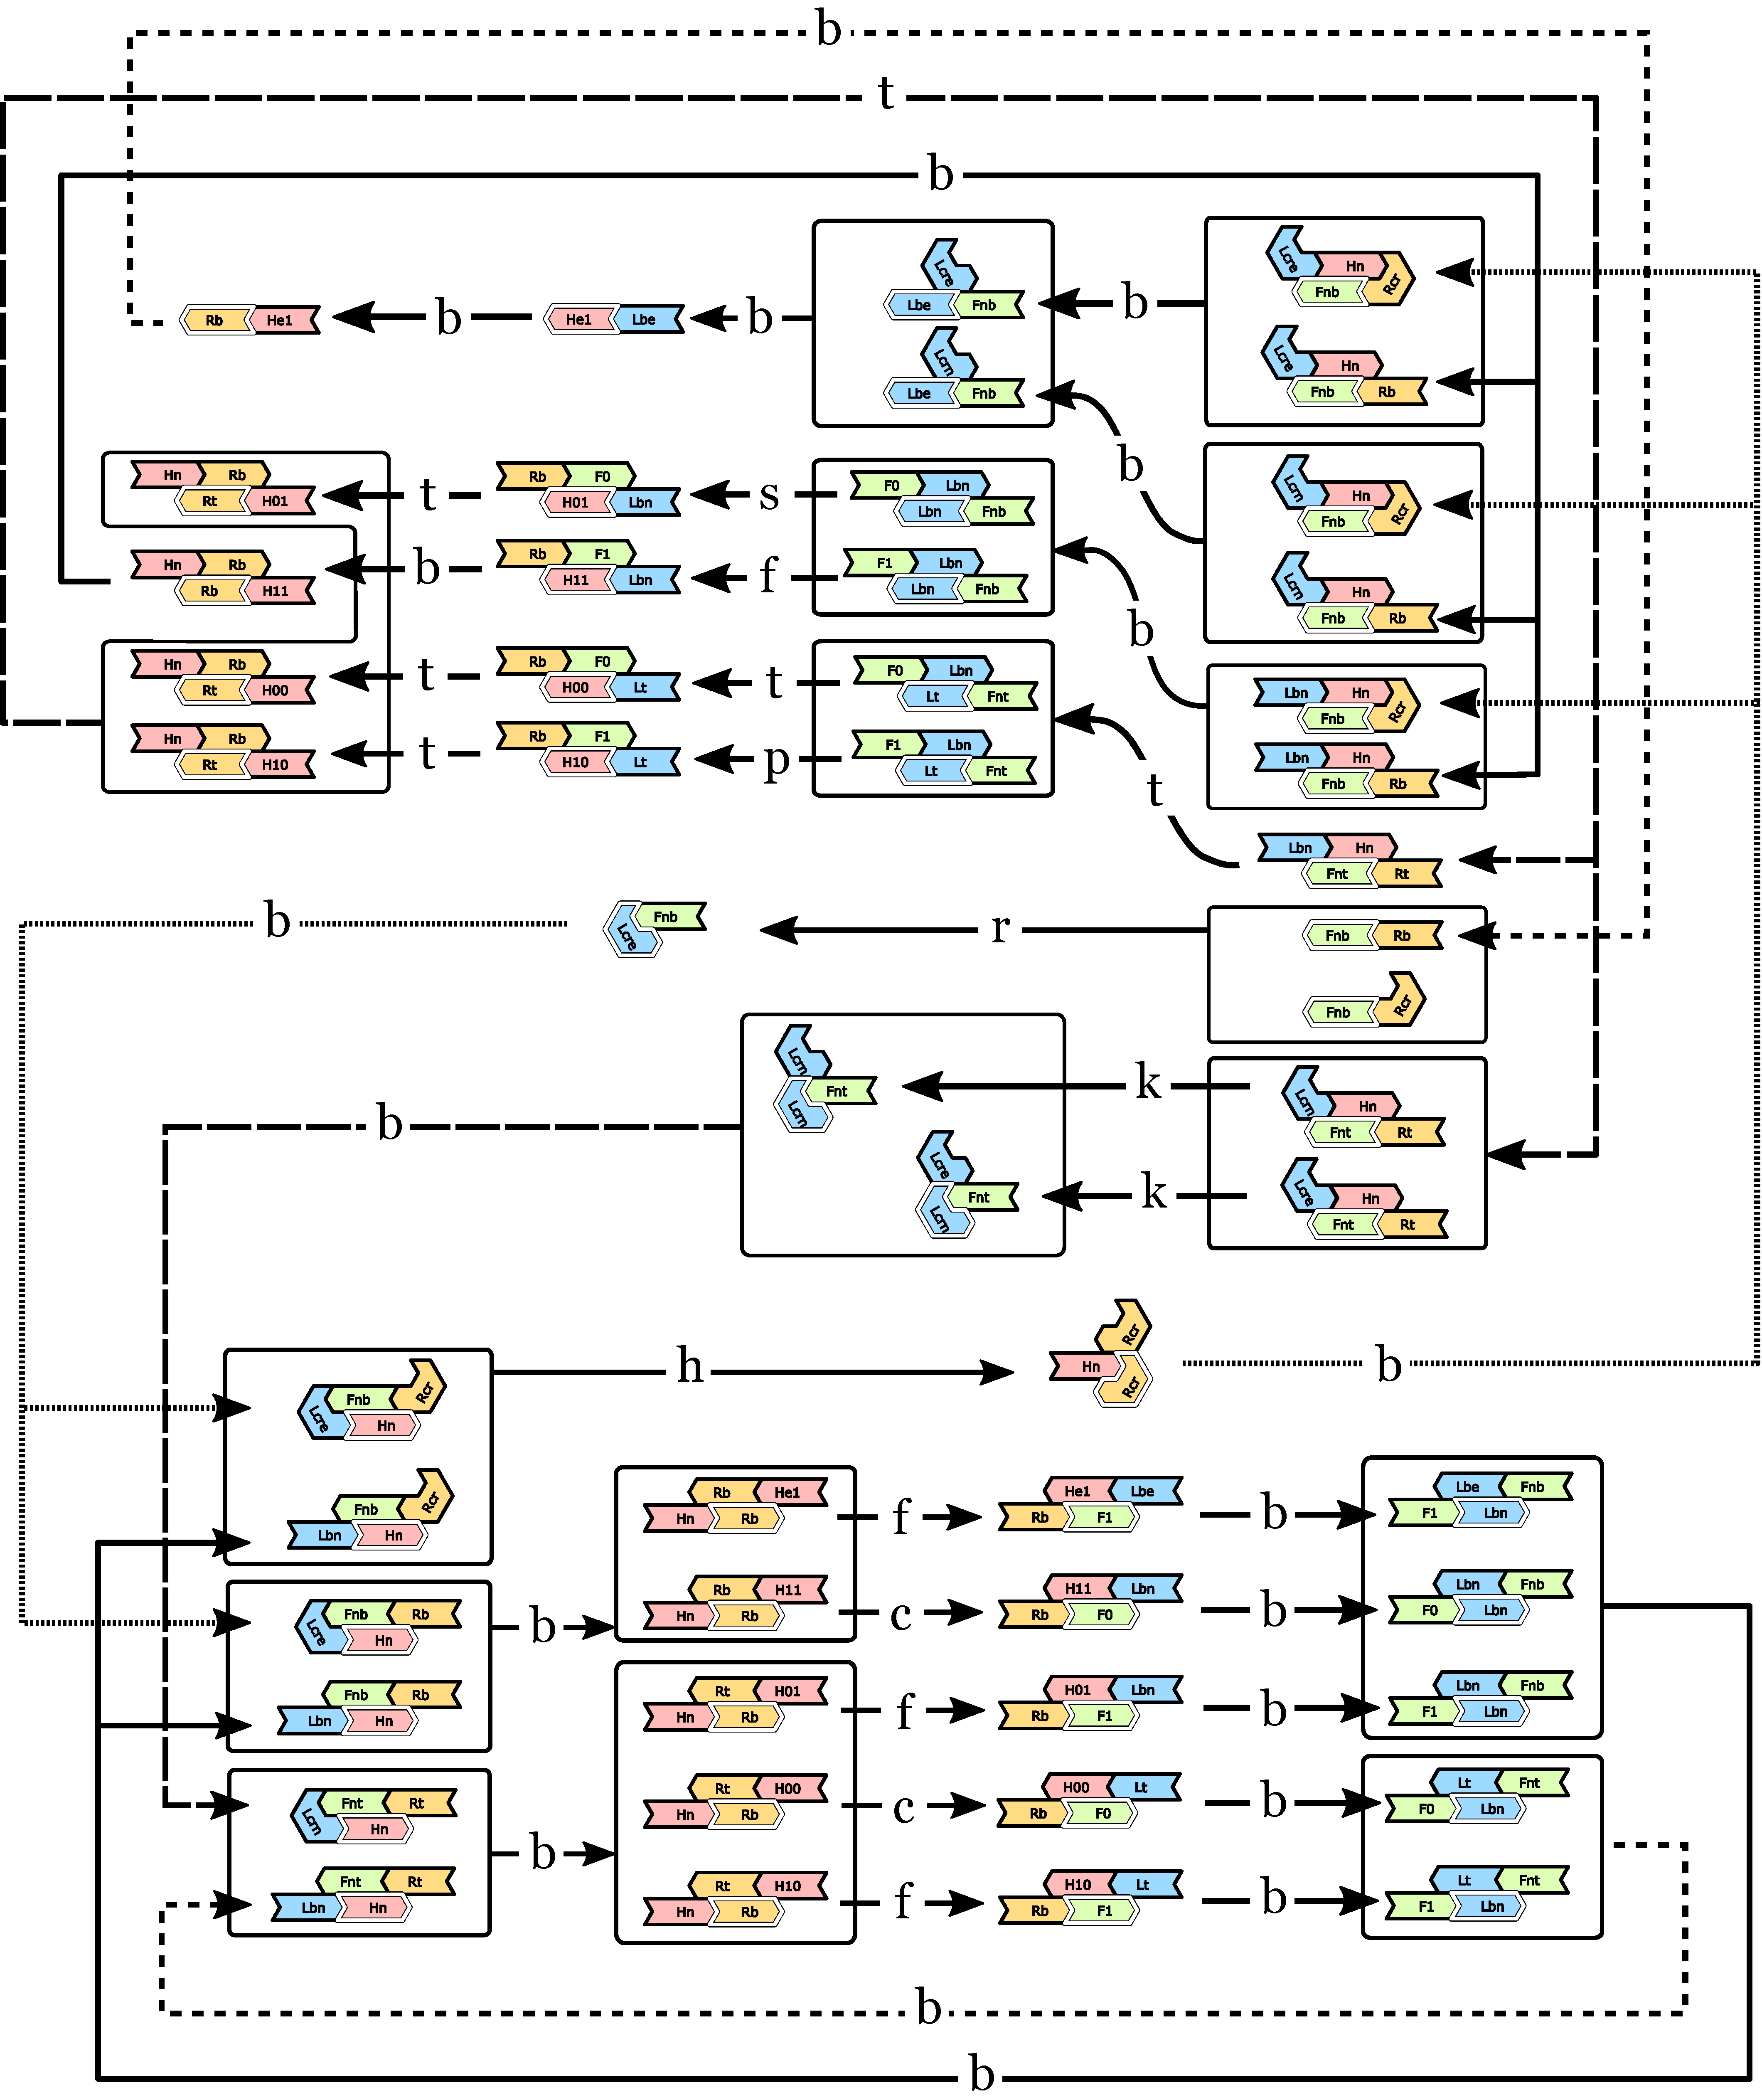
\includegraphics[width=0.9\textwidth]{fig/svg/inf-ai_c_2.pdf}
\vspace*{5mm}

\scalebox{0.7}{
\begin{tikzpicture}
	\node[anchor=north, inner sep=0] (tg) at (0,0) {
 		   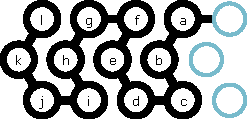
\includegraphics[width=0.15\textwidth]{fig/svg/tglider.pdf}
	};
	\node[anchor=north, inner sep=0] (bg) at (3,0) {
 		   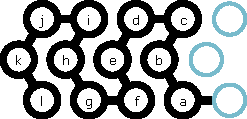
\includegraphics[width=0.15\textwidth]{fig/svg/bglider.pdf}
	};
	\node[anchor=north, inner sep=0] (pl) at (6,0) {
 		   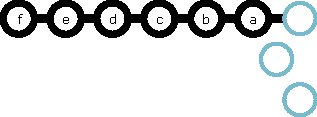
\includegraphics[width=0.15\textwidth]{fig/svg/plane.pdf}
	};
	\node[anchor=north, inner sep=0] (sp) at (9,0) {
 		   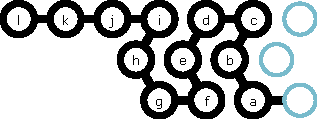
\includegraphics[width=0.15\textwidth]{fig/svg/spiral.pdf}
	};
	
	\node[anchor=north, inner sep=0] (ho) at (-1.5,-3) {
 		   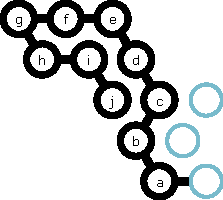
\includegraphics[width=0.15\textwidth]{fig/svg/horn.pdf}
	};
	\node[anchor=north, inner sep=0] (ka) at (1.5,-3) {
 		   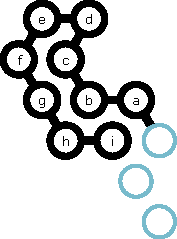
\includegraphics[width=0.12\textwidth]{fig/svg/kar.pdf}
	};
	\node[anchor=north, inner sep=0] (ro) at (4.5,-3) {
 		   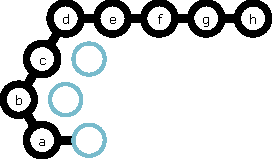
\includegraphics[width=0.15\textwidth]{fig/svg/roof.pdf}
	};
	\node[anchor=north, inner sep=0] (fa) at (7.5,-3) {
 		   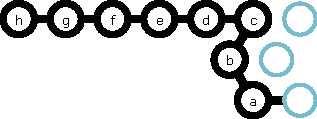
\includegraphics[width=0.2\textwidth]{fig/svg/fault.pdf}
	};
	\node[anchor=north, inner sep=0] (ci) at (10.5,-3) {
 		   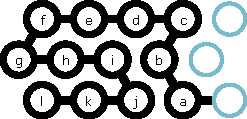
\includegraphics[width=0.2\textwidth]{fig/svg/cliff.pdf}
	};
	
	\node[below, shift=(-90:0.8)] at (tg) {t};
	\node[below, shift=(-90:0.8)] at (bg) {b};
	\node[below, shift=(-90:0.8)] at (pl) {p};
	\node[below, shift=(-90:0.8)] at (sp) {s};

	\node[below, shift=(-90:1)] at (ho) {h};
	\node[below, shift=(-90:1)] at (ka) {k};
	\node[below, shift=(-90:0.8)] at (ro) {r};
	\node[below, shift=(-90:0.8)] at (fa) {f};
	\node[below, shift=(-90:0.8)] at (ci) {c};
\end{tikzpicture}
}
\caption{The brick automaton of infinite binary counter}
\label{fig:brickautomaton}
\end{figure*}


%%%%%%

\begin{figure}[tb]
\begin{tabular}{c}
 \begin{minipage}{0.5\linewidth}
  \centering
   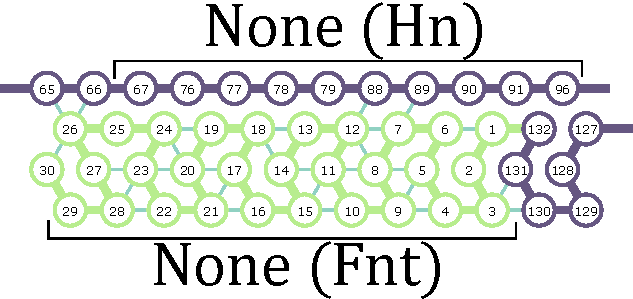
\includegraphics[width=0.7\linewidth]{fig/svg/Fnt_1.pdf}
 \end{minipage}
 
 \begin{minipage}{0.5\linewidth}
  \centering
   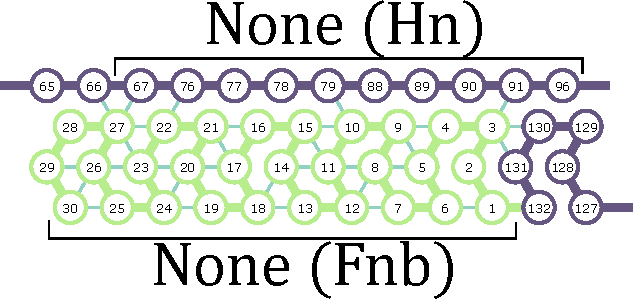
\includegraphics[width=0.7\linewidth]{fig/svg/Fnb_1.pdf}

 \end{minipage}
 \end{tabular}
\ \\
\ \\
\begin{tabular}{c}
 \begin{minipage}{0.5\linewidth}
  \centering
   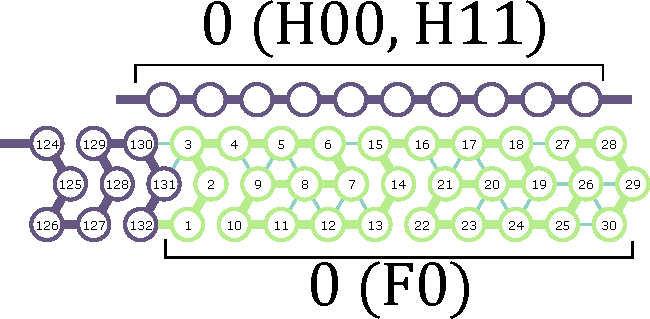
\includegraphics[width=0.7\linewidth]{fig/svg/F0_1.pdf}
 \end{minipage}
 
 \begin{minipage}{0.5\linewidth}
  \centering
   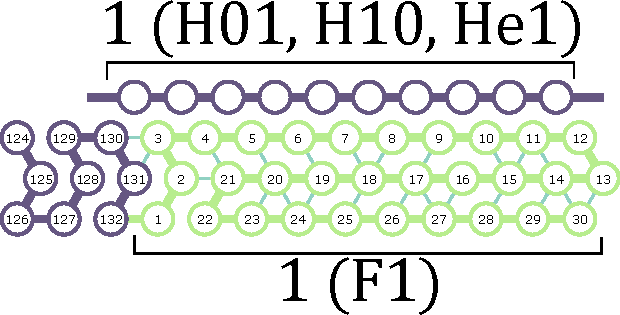
\includegraphics[width=0.7\linewidth]{fig/svg/F1_1.pdf}

 \end{minipage}
 \end{tabular}
 \caption{All the four bricks of module F: The two bricks at the top, \texttt{Fnt} and \texttt{Fnb}, are for zigs while the others, \texttt{F0} and \texttt{F1}, are for zags. }
 \label{fig:formatters}
\end{figure}

%%

%%

\begin{figure}[tb]
\begin{tabular}{c}
 \begin{minipage}{0.5\linewidth}
  \centering
   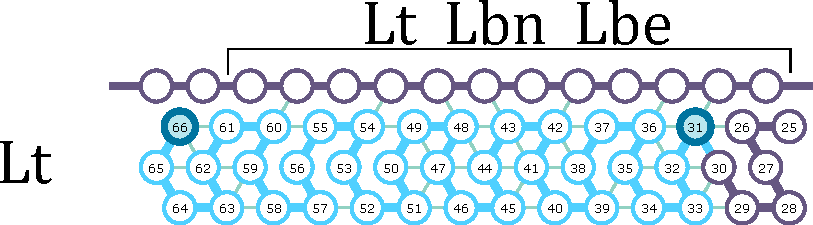
\includegraphics[width=0.9\linewidth]{fig/svg/Lt_3.pdf}
 \end{minipage}
 
 \begin{minipage}{0.5\linewidth}
  \centering
   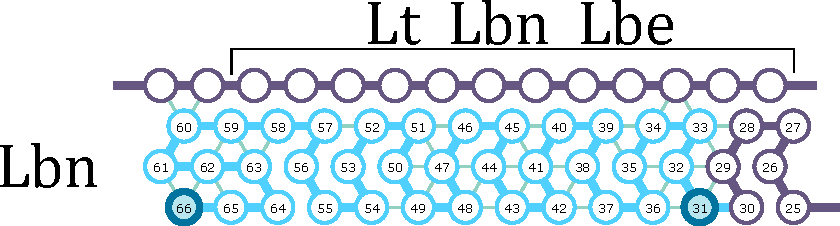
\includegraphics[width=0.9\linewidth]{fig/svg/Lbc_3.pdf}

 \end{minipage}
 \end{tabular}

\vspace*{3mm}

\begin{tabular}{c}
 \begin{minipage}{0.5\linewidth}
  \centering
   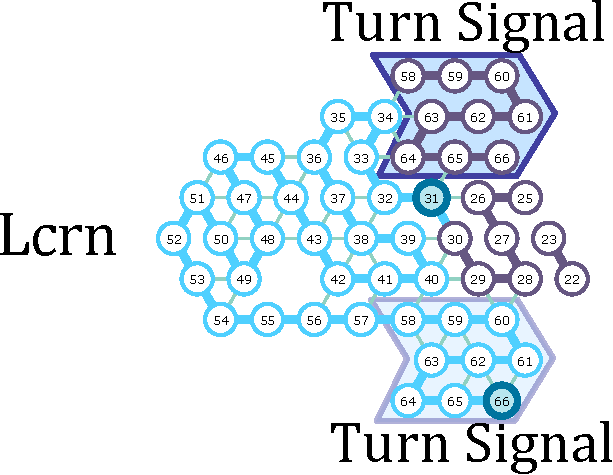
\includegraphics[width=0.8\linewidth]{fig/svg/Ltrc_3.pdf}
 \end{minipage}
 
  \begin{minipage}{0.5\linewidth}
  \centering
   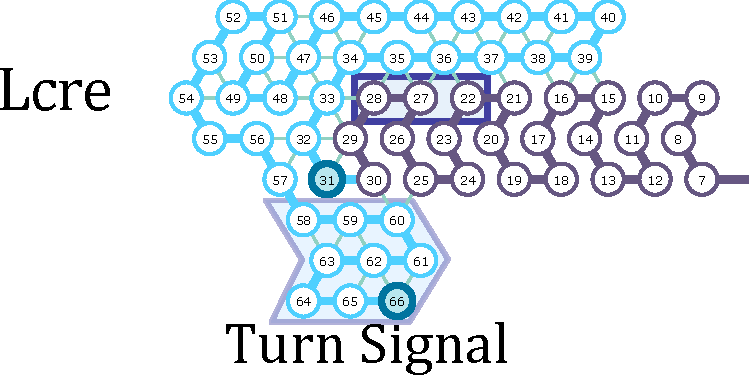
\includegraphics[width=\linewidth]{fig/svg/Ltre_3.pdf}
 \end{minipage}
 \end{tabular}

  \centering
   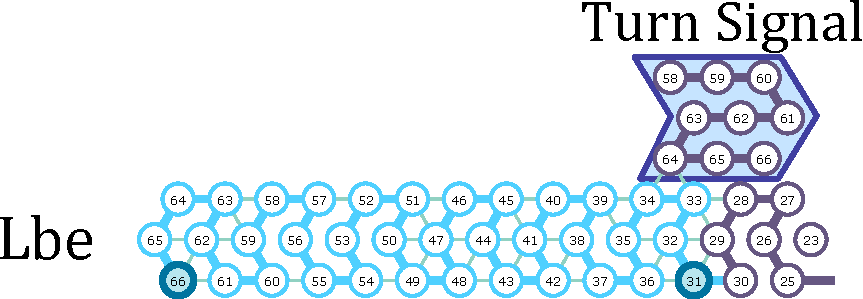
\includegraphics[width=0.5\linewidth]{fig/svg/Lbe_3.pdf}


 
 \caption{All the five bricks of module L: \texttt{Lt}, \texttt{Lbn}, \texttt{Lcrn}, \texttt{Lcre}, and \texttt{Lbe} from top left to bottom right.
In zigs, L folds into either \texttt{Lt} or \texttt{Lbn} depending on where it starts, until the transcript reaches the left end, where L folds either into \texttt{Lcrn} if the current value has not been overflowed, or into \texttt{Lbe} at an overflow.
In the case of overflow, the next L folds into \texttt{Lcre}.
In zags, L always folds into \texttt{Lbn}.}
 \label{fig:leftturns}
\end{figure}

\section{Folding an infinite binary counter}

%チューリングマシンがbead type 542で今回は132

%\subsection{General idea}
%\paragraph{General idea.}
Between two consecutive overflows, the proposed system behaves in the same way as the finite binary counter proposed by Geary et al. \cite{GeMeScSe2019}.
Its transcript folds in a zigzag manner macroscopically (downward in figures throughout this paper).
A zig, folding from right to left, increments the current value of the counter by 1.
The succeeding zag, folding from left to right, formats the incremented value for the sake of next zig and copies it downward.
Unlike the existing counter, when a zig encounters an overflow, it does not abort but rather extends the current value by 1 bit.

%Each zig or zag is 3-rows thick.
%Each pass extends to straight while folding into glider and folds its last module folds into turn module and starts next pass.


The transcript of our counter is periodic.
Its period \texttt{1}-\texttt{2}-\texttt{3}- $\cdots$ -\texttt{132} is semantically divided into the following four subsequences, called \textit{modules}:
\texttt{1}--\texttt{30} (Format module or F; colored in green in figures),
\texttt{31}--\texttt{66} (Left-Turn module or L; blue),
\texttt{67}--\texttt{96} (Half-Adder module or H; red),
and \texttt{97}--\texttt{132} (Right-Turn module  or R; yellow).
%\begin{itemize}
%\item \texttt{1}--\texttt{30}: Format module or F
%\item \texttt{31}--\texttt{66}: Left-Turn module or L
%\item \texttt{67}--\texttt{96}: Half-Adder module or H
%\item \texttt{97}--\texttt{132}: Right-Turn module  or R
%\end{itemize}
The transcript can be hence represented as $(FLHR)^*$ at the module level. Modules are to play their roles in expected environments by folding into respective conformations which should be pairwise-distinct enough to be distinguishable by other modules transcribed later.
Such expected conformations are called a \textit{brick}.
For example, module F encounters the four environments shown in Fig.~\ref{fig:formatters} where it takes the four bricks \texttt{Fnt}, \texttt{Fnb}, \texttt{F0}, and \texttt{F1}, respectively.
Here, by saying (an instance of) a module folds into (or takes) a brick in an environment, what we actually mean is that the rule set is designed so as for the transcript of the module to interact with itself as well as with the environment into that brick according to the oritatami dynamics  \eqref{eq:OS_CF}.
The whole system is designed to guarantee that each module is transcribed only in one of the environments it expects.
This fact is illustrated in the \textit{brick automaton}, which describes pairs of an environment and a brick as a vertex and transitions between them.
Since this automaton is closed, it suffices to test whether for all pairs of an environment and a brick, the brick is folded in the environment.
This test has been done \textit{in-silico} using our simulator developed for this project.
This brick automaton and all the certificates can be found at \href{https://komaruyama.github.io/oritatami-infinit-counter/}{\texttt{https://komaruyama.github.io/oritatami-infinit-counter/}}.

\begin{figure}[tb]
\begin{tabular}{c}
 \begin{minipage}{0.33\linewidth}
  \centering
   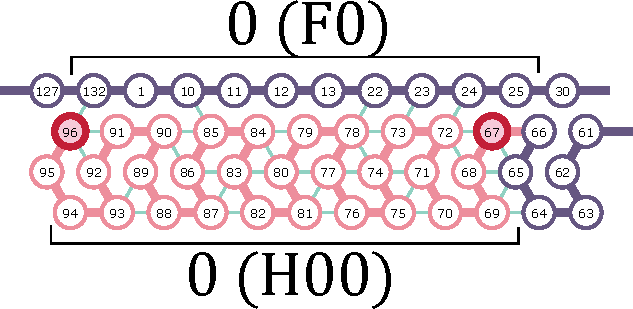
\includegraphics[width=0.9\linewidth]{fig/svg/H00_1.pdf}
 \end{minipage}
 
 \begin{minipage}{0.33\linewidth}
  \centering
   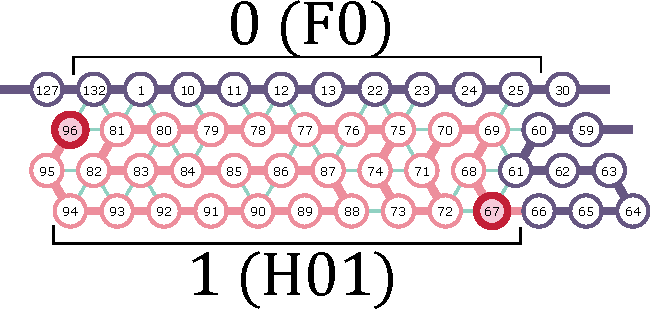
\includegraphics[width=0.9\linewidth]{fig/svg/H01_1.pdf}

 \end{minipage}
 
  \begin{minipage}{0.33\linewidth}
  \centering
   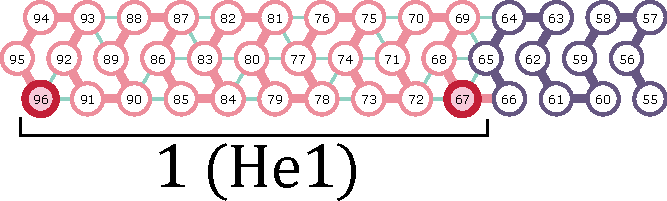
\includegraphics[width=0.9\linewidth]{fig/svg/He1_1.pdf}
 \end{minipage}
 \end{tabular}

\begin{tabular}{c}
\ \\
 \begin{minipage}{0.33\linewidth}
  \centering
   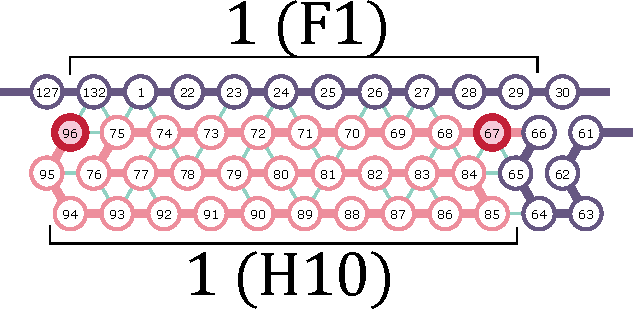
\includegraphics[width=0.9\linewidth]{fig/svg/H10_1.pdf}
 \end{minipage}
 
 \begin{minipage}{0.33\linewidth}
  \centering
   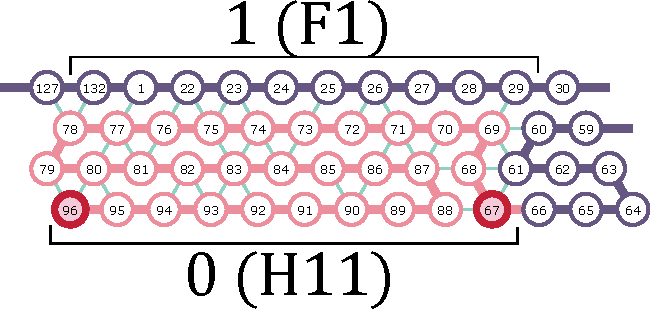
\includegraphics[width=0.9\linewidth]{fig/svg/H11_1.pdf}
 \end{minipage}
 
  \begin{minipage}{0.33\linewidth}
  \centering
   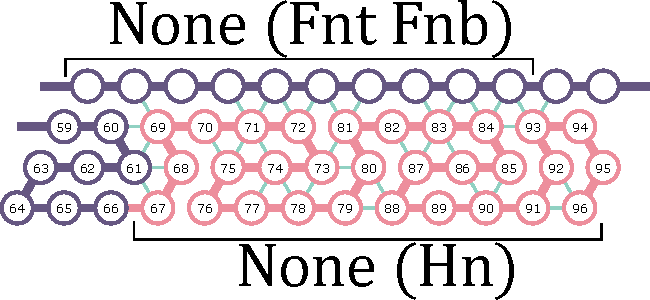
\includegraphics[width=0.9\linewidth]{fig/svg/Hn_1.pdf}

 \end{minipage}
 \end{tabular}
 \caption{All the six bricks of module H: \texttt{H00}, \texttt{H01}, \texttt{He1}, \texttt{H10}, \texttt{H11}, and \texttt{Hn} from top left to bottom right.
In zags, H always folds into \texttt{Hn} while in zigs, it folds into one of the other five bricks.}
 \label{fig:halfadders}
\end{figure}


\begin{figure}[tb]
\begin{tabular}{c}
 \begin{minipage}{0.5\linewidth}
  \centering
   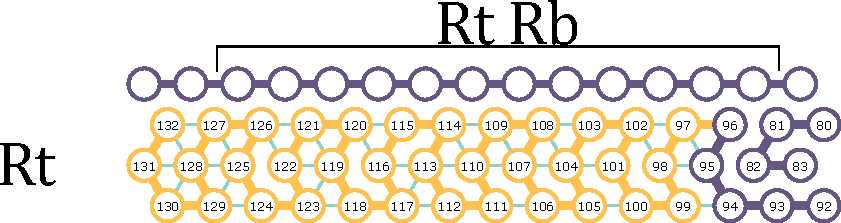
\includegraphics[width=0.8\linewidth]{fig/svg/Rt_1.pdf}\\
   \vspace*{3mm}
   
   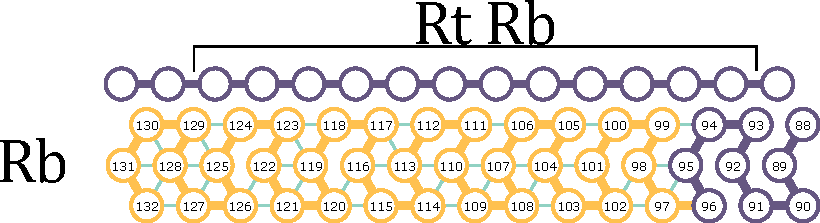
\includegraphics[width=0.8\linewidth]{fig/svg/Rb_1(2).pdf}\\
   \vspace*{2mm}
   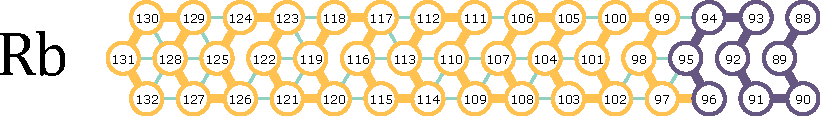
\includegraphics[width=0.8\linewidth]{fig/svg/Rb_1.pdf}
 \end{minipage}
 
 \begin{minipage}{0.5\linewidth}
  \centering
   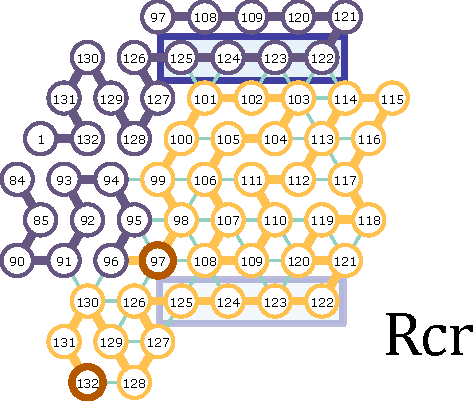
\includegraphics[width=0.7\linewidth]{fig/svg/Rtr_1.pdf}
 \end{minipage}
 \end{tabular}

 \caption{All the three bricks of module R: \texttt{Rt}, \texttt{Rb}, and \texttt{Rcr}.
 In zigs, R folds into \texttt{Rt} or \texttt{Rb}, depending on how high it starts.
 In zags, R always folds into \texttt{Rb} until the transcript reaches the right end, where R folds into \texttt{Rcr}.}
 \label{fig:rightturns}
\end{figure}

\paragraph{Seed and Encoding.}
The initial counter value is encoded as $b_{k-1}b_{k-2} \cdots b_1b_0$ in binary on the seed in the following format
\begin{equation} \label{eq:zagencoding}
\texttt{64}{-}\texttt{65}{-}\texttt{66}{-}\left( \prod^0_{i = k-1} \bigl(  w_{Hn} w_{Rb} w_{Fb_i} w_{Lbn} \bigr) \right) w_{Hn}
\end{equation}
where 
\begin{eqnarray*}
w_{Hn} &=& \texttt{67}{-}\texttt{76}{-}\texttt{77}{-}\texttt{78}{-}\texttt{79}{-}\texttt{88}{-}\texttt{89}{-}\texttt{90}{-}\texttt{91}{-}\texttt{96},\\
w_{Rb} &=& \texttt{97}{-}\texttt{102}{-}\texttt{103}{-}\texttt{108}{-}\texttt{109}{-}\texttt{114}{-}\texttt{115}{-}\texttt{120}{-} \\
& & {-}\texttt{121}{-}\texttt{126}{-}\texttt{127}{-}\texttt{132},\\
w_{F0} &=& \texttt{1}{-}\texttt{10}{-}\texttt{11}{-}\texttt{12}{-}\texttt{13}{-}\texttt{22}{-}\texttt{23}{-}\texttt{24}{-}\texttt{25}{-}\texttt{30},\\
w_{F1} &=& \texttt{1}{-}\texttt{22}{-}\texttt{23}{-}\texttt{24}{-}\texttt{25}{-}\texttt{26}{-}\texttt{27}{-}\texttt{28}{-}\texttt{29}{-}\texttt{30},\\
 w_{Lbn} &=& \texttt{31}{-}\texttt{36}{-}\texttt{37}{-}\texttt{42}{-}\texttt{43}{-}\texttt{48}{-}\texttt{49}{-}\texttt{54}{-}\texttt{55}{-}\texttt{64}{-}\texttt{65}{-}\texttt{66}.
\end{eqnarray*}
$w_{Hn}$, $w_{Rb}$, $w_{F0}$, $w_{F1}$, and $w_{Lbn}$ are sequences of bead types exposed downward by modules H, R, F, L when they fold into bricks \texttt{Hn}, \texttt{Rb}, \texttt{F}$b_i$, \texttt{Lbn}, respectively, which can be found in Figs.~\ref{fig:halfadders}, \ref{fig:rightturns}, \ref{fig:formatters}, and \ref{fig:leftturns}.
%For example, $w_{Hn} = \texttt{67}{-}\texttt{76}{-}\texttt{77}{-}\texttt{78}{-}\texttt{79}{-}\texttt{88}{-}\texttt{89}{-}\texttt{90}{-}\texttt{91}{-}\texttt{96}$.
The seed is exemplified for $k = 1$ and $b_0 = 0$ in Fig.~\ref{fig:counter1stzig}, where it is colord in purple.
%$w_{Hn} = 67{-}76{-}77{-}78{-}79{-}88{-}89{-}90{-}91{-}96$ \\
%$w_{Rb} = 97{-}102{-}103{-}108{-}109{-}114{-}115{-}120{-}121{-}126{-}127{-}132$\\
%$w_{Lbn} = 31{-}36{-}37{-}42{-}43{-}48{-}49{-}54{-}55{-}64{-}65{-}66$

%\subsection{Brick level overview}
\paragraph{Brick level overview}
Starting from the seed, this system cyclically transits four phases: zig ($\leftarrow$), left carriage-return ($\hookrightarrow$), zag ($\rightarrow$), and right carriage-return ($\hookleftarrow$). 
The prefix $(FLHR)^k F$ of the transcript folds into the first zig (recall that $k$ is the bit-width of the initial value). 
In zigs in general, all the instances of modules F and H fold into bricks of width 10 and height 3, while all the instances of  L and R fold into bricks of width 12 and height 3. 
Zigs thus turn out to be a linear structure of height 3. 
We can inductively observe that the $i$-th instance of H in the prefix is transcribed right below $b_{i-1}$ encoded on the seed in the format (2) so that the H can ``read" $b_{i-1}$. 
After the whole prefix thus has folded into the first zig, the next L is transcribed right below Turn Signal, which lets the L fold into a special brick for left carriage-return if the zig ended at the top (this occurs when $b_{k-1} b_{k-2} \cdots b_0 < 1^k$) (see Fig.~\ref{fig:counter1stzag}). 
We should note that this special brick \texttt{Lcre} is provided with another Turn Signal for the sake of next left carriage-return.
Having been thus carriage-returned, the succeeding subsequence $(HRFL)^k H$ of the transcript folds into the first zag.
Even in zags instances of F and H fold into bricks of width 10 and height 3, while those of L and R fold into bricks of width 12 and height 3. 
As a result, zags turn out to be a linear structure of height 3. 
More importantly, instances of H and F are aligned thus vertically and alternately into columns (see Figs.~\ref{fig:counter1stzig}-\ref{fig:overflowex1}), $i$-th of which from the right propagates the ($i{-}1$)-th bit of the counter value downward. 
After the whole subsequence has folded into the first zag, an instance of $R$ is transcribed and folded into a special brick \texttt{Rcr} for right carriage-return due to the turn signal \texttt{125}-\texttt{124}-\texttt{123}-\texttt{122}, which occurs also at the bottom of \texttt{Rcr} for the sake of next right carriage-return. 
This amounts to one cycle of the phase transition.
 

%\subsection{Increment of the counter}
\paragraph{Increment of the counter}
In a zig, module H plays its primary role as a half-adder and carry transfers through instances of others (F, L, and R) from an instance of H to another for more significant bit.
Carry transfers as a height for modules to start.
In zigs, modules F, L, and R take the respective two bricks (\texttt{Fnt} and \texttt{Fnb} for F, \texttt{Lt} and \texttt{Lbn} for L, and \texttt{Rt} and \texttt{Rb} for R; see Figs.~\ref{fig:formatters}, \ref{fig:leftturns}, and \ref{fig:rightturns}), both of which start and end at the same height: one at the top while the other at the bottom.
A zig is carried by being forced to start at the bottom by the last \texttt{Rcr} or the seed.
Until the count overflows, module H encounters only four environments, which encode input 0 as $w_{F0}$ or 1 as $w_{F1}$ and carry or no-carry as of whether the module starts at the bottom or top, where it takes \texttt{H00}, \texttt{H01}, \texttt{H10}, and \texttt{H11}, respectively, as shown in Fig.~\ref{fig:halfadders} (\texttt{H}$xc$ is folded when the input is $x$ and the carry is given if $c=1$ or not otherwise).

\begin{figure}[tb]
\centering
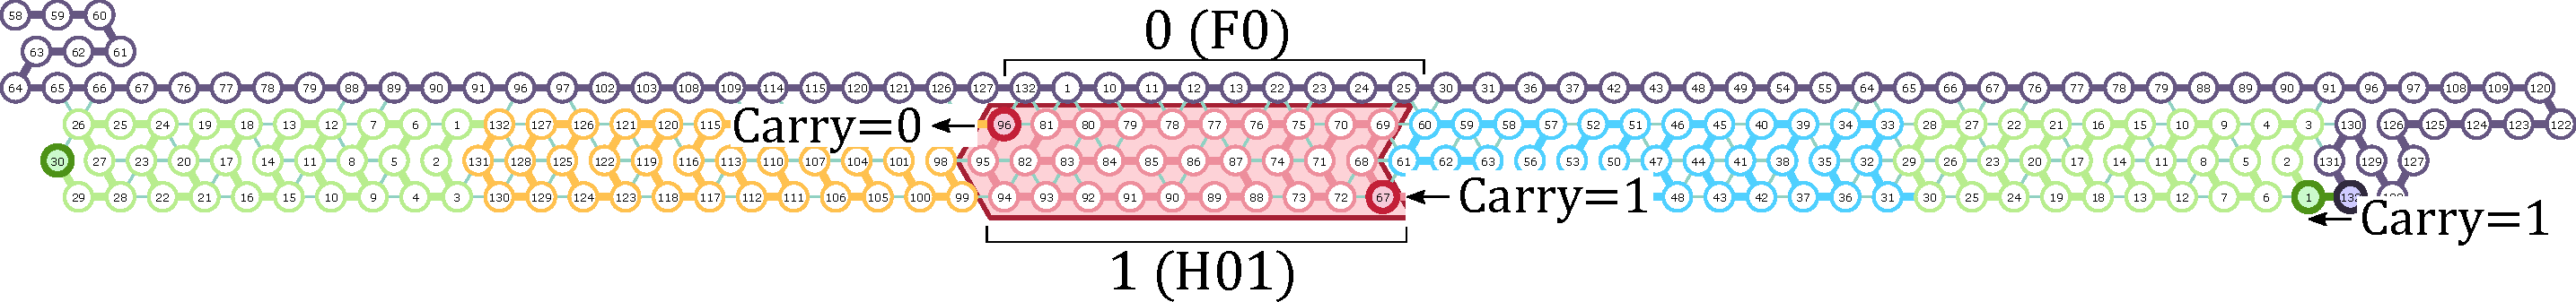
\includegraphics[width=\linewidth]{fig/svg/CounterEx5_1.pdf}
\caption{
The first zig.
0 is encoded as an initial value below the seed in the format \eqref{eq:zagencoding} with $k = 1$ (1-bit width).
Being fed with carry, the zig increments the value.
Module H outputs 1, or more precisely a sequence of bead types which shall be interpreted as 1 in the next zag and reformatted, as a sum and cancels the carry.
}
%\textcircled{\scriptsize 1}{-}\textcircled{\scriptsize 10}{-}\textcircled{\scriptsize 11}{-}\textcircled{\scriptsize 12}{-}\textcircled{\scriptsize 13}{-}\textcircled{\scriptsize 22}{-}\textcircled{\scriptsize 23}{-}\textcircled{\scriptsize 24}{-}\textcircled{\scriptsize 25}{-}\textcircled{\scriptsize 30},

\label{fig:counter1stzig}
\end{figure}

\begin{figure}[tb]
\centering
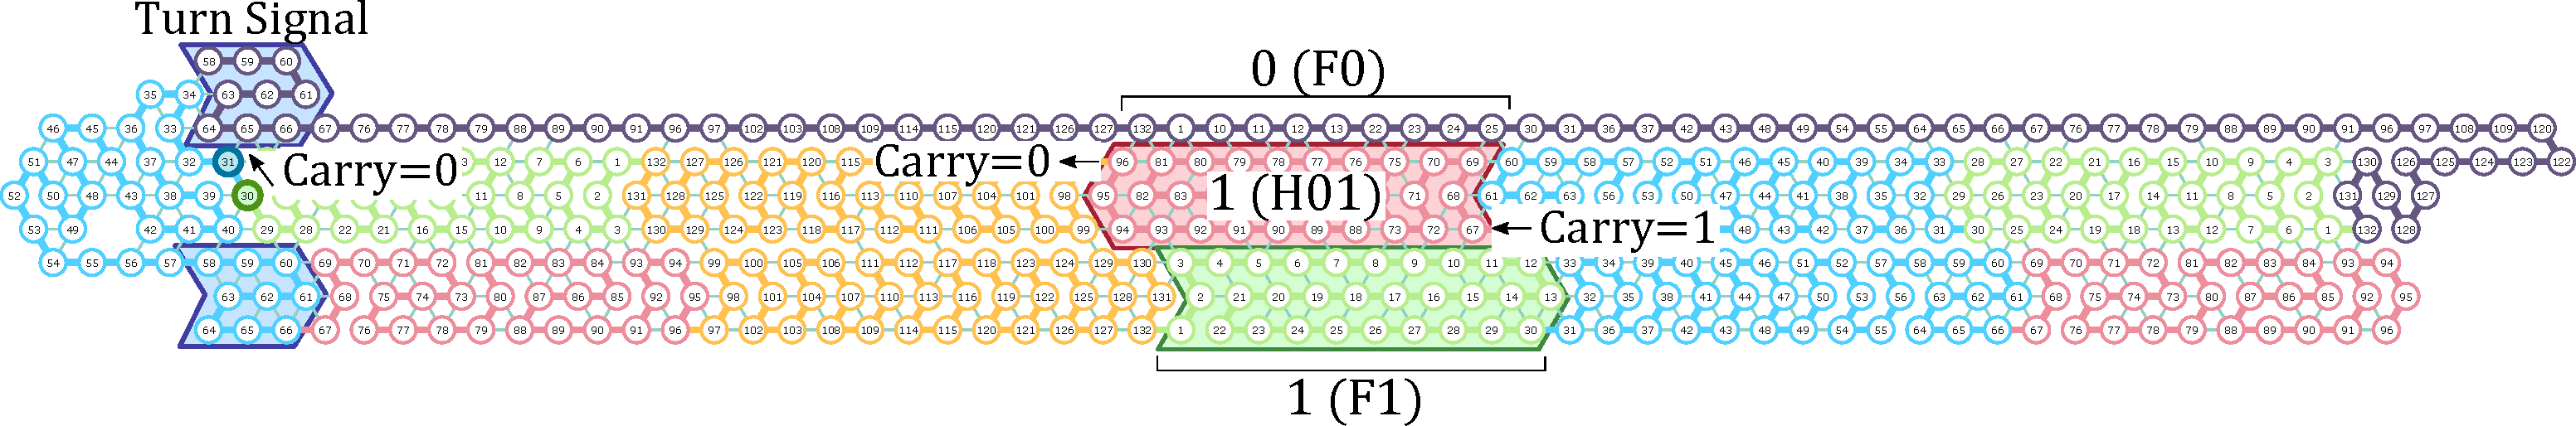
\includegraphics[width=\linewidth]{fig/svg/CounterEx11_1.pdf}
\caption{
Module L turns and start the first zag pass.
Since there is a Turn Signal at the left end of the seed, when the carry is 0, module L turns and at the end of L forms Turn Signal.
In zag pass, module F reads the output of module H and copies it down,
}
\label{fig:counter1stzag}
\end{figure}

\begin{figure}[tb]
\centering
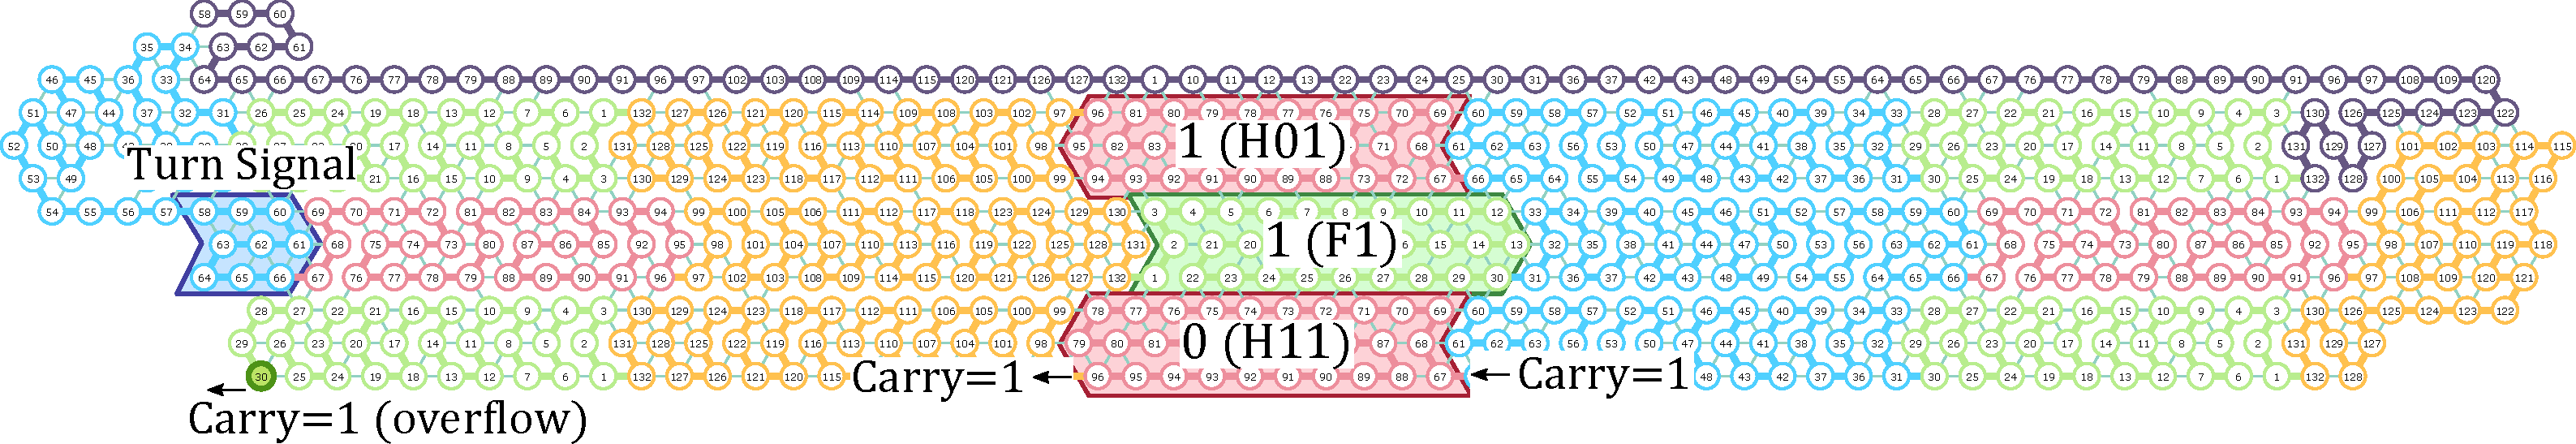
\includegraphics[width=\linewidth]{fig/svg/CounterEx13_1.pdf}
\caption{
Reach the left end with carry.
Even if transcript of module L sticks to Turn Signal, it can not bind because the distance is long.
}
\label{fig:overflowex1}
\end{figure}

Let us see how the subsequence $(FLHR)^kF$ folds into a zig in order to count up; for $k=1$ and the current value 0, see Fig.~\ref{fig:counter1stzig}.
The zig starts at the bottom, that is, being carried, and the carry transfers through the first instances of F and L in the way just explained toward the first instance of H.
This H is thus fed with carry and folds into \texttt{H01} if the bit encoded above is 0, as illustrated in Fig.~\ref{fig:counter1stzig}, or \texttt{H11} if the bit is rather 1.
\texttt{H01} ends at the top, corresponding to canceling the carry out.
This absence of carry transfers through the succeeding modules leftward.
As a result, the zig ends, or more precisely an instance of F ends folding at the bottom if the current value is overflowed (Fig.~\ref{fig:overflowex1}), or at the top otherwise (Fig.~\ref{fig:counter1stzig}).
An instance of L is to be transcribed next.
It folds either into \texttt{Lcrn} for (normal) carriage-return unless the current value is overflowed, or into \texttt{Lbe} at an overflow.


%\subsection{Bit width expansion at an overflow}
\paragraph{Bit-width expansion at an overflow}
The counter of Geary et al. cannot handle a zig that ends at the bottom, that is, its behavior is undefined at an overflow.
In contrast, module L in this infinite counter is designed so as to fold into \texttt{Lbe} in this situation in order to continue counting up (Fig.~\ref{fig:overflowex2-3}).
Observe that the dent on Turn Signal made of \texttt{58}, \texttt{63}, and \texttt{64} is too far for module L or more precisely its beads \texttt{33} and \texttt{34} to interact with strongly enough to fold into \texttt{Lcrn}.
\texttt{Lbe} is a self-sustaining conformation (glider) so that it can fold even if nothing is around, which occurs at that very moment.
For the same reason, the following instances of H, R, and F fold into self-sustaining conformations \texttt{He1}, \texttt{Rb}, and \texttt{Fnb}, respectively (Figs.~\ref{fig:overflowex2-3} and \ref{fig:overflowex4}).
%If the beads \texttt{33} and \texttt{34} bind to Turn Signal, module L folds into \texttt{Lcrn}, but now, these beads cannot reach to Turn Signal because module L is starting at the bottom.
Note that \texttt{He1} is essentially the same as \texttt{H00} but exposes the opposite side downward, which will be interpreted as the leading bit 1 after expansion in the next zag.
When the next instance of L is transcribed, there is nothing around.
Nevertheless, it does not fold into \texttt{Lbe} but folds into \texttt{Lcre} for carriage-return; how?
It is guided by interaction between the beads \texttt{35}, \texttt{36} along the transcript of L and the Turn Signal \texttt{28}{-}\texttt{27}{-}\texttt{22} above \texttt{Fnb} (Figs.~\ref{fig:leftturns} and \ref{fig:overflowex4}).
This signal is usually hidden geometrically by the previous zag, and hence, does no harm.


%\subsection{Formatting}
\paragraph{Formatting}
The value has been successfully incremented but it is not in the format \eqref{eq:zagencoding} yet.
In the upcoming zag, instances of F play their primary role to format 1 bit output by module H (recall that instances of H and F are aligned vertically and alternately).
Both of the bricks of L for carriage-return, i.e., \texttt{Lcrn} and \texttt{Lcre}, end at the bottom so that zags start at the bottom.
All modules start and end at the bottom in zags; note that nothing has to be transferred between modules.
That is, instances of H, L, and R fold into \texttt{Hn}, \texttt{Lbn}, and \texttt{Rb}, respectively.
Below the brick \texttt{H}$xc$, an instance of F folds into \texttt{F}$y$, where $y = (x+c) \mod 2$.

%
%Here, the value incremented in the previous zig is formatted so as to be exposed below in the format \eqref{eq:zagencoding} for the next zig.
%A subsequence $(HRFL)^kH$ of the transcript folds into the zag, where $k$ is the bit width of the incremented value.
%Both of the bricks of L for carriage-return, i.e., \texttt{Lcrn} and \texttt{Lcre}, ends at the bottom so that zags start at the bottom.
%The first instances of H and R fold into \texttt{Hn} and \texttt{Rb}, respectively.
%Hence, the next F starts at the bottom and takes the brick \texttt{F}$y$ under the module H  that takes the brick \texttt{H}$xc$ in the previous zig, where $y$ is the output of the module, that is, $y = (x+c) \mod 2$.
%Both of these bricks \texttt{F0} and \texttt{F1} end at the bottom so that the instance of L folds into \texttt{Lbn}.


\begin{figure}[tb]
\begin{tabular}{c}
 \begin{minipage}{0.35\linewidth}
\centering
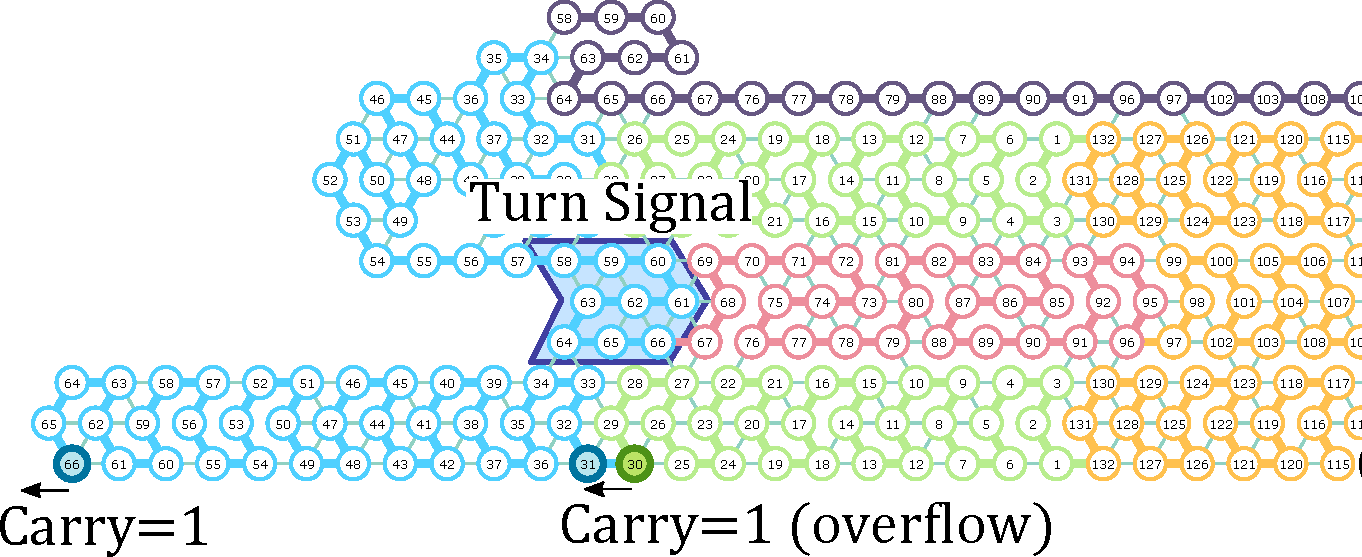
\includegraphics[width=\linewidth]{fig/svg/CounterEx14_2.pdf}
\end{minipage}
\begin{minipage}{0.05\linewidth}
\centering
{\large $\Rightarrow$}
\end{minipage}
 \begin{minipage}{0.55\linewidth}
\centering
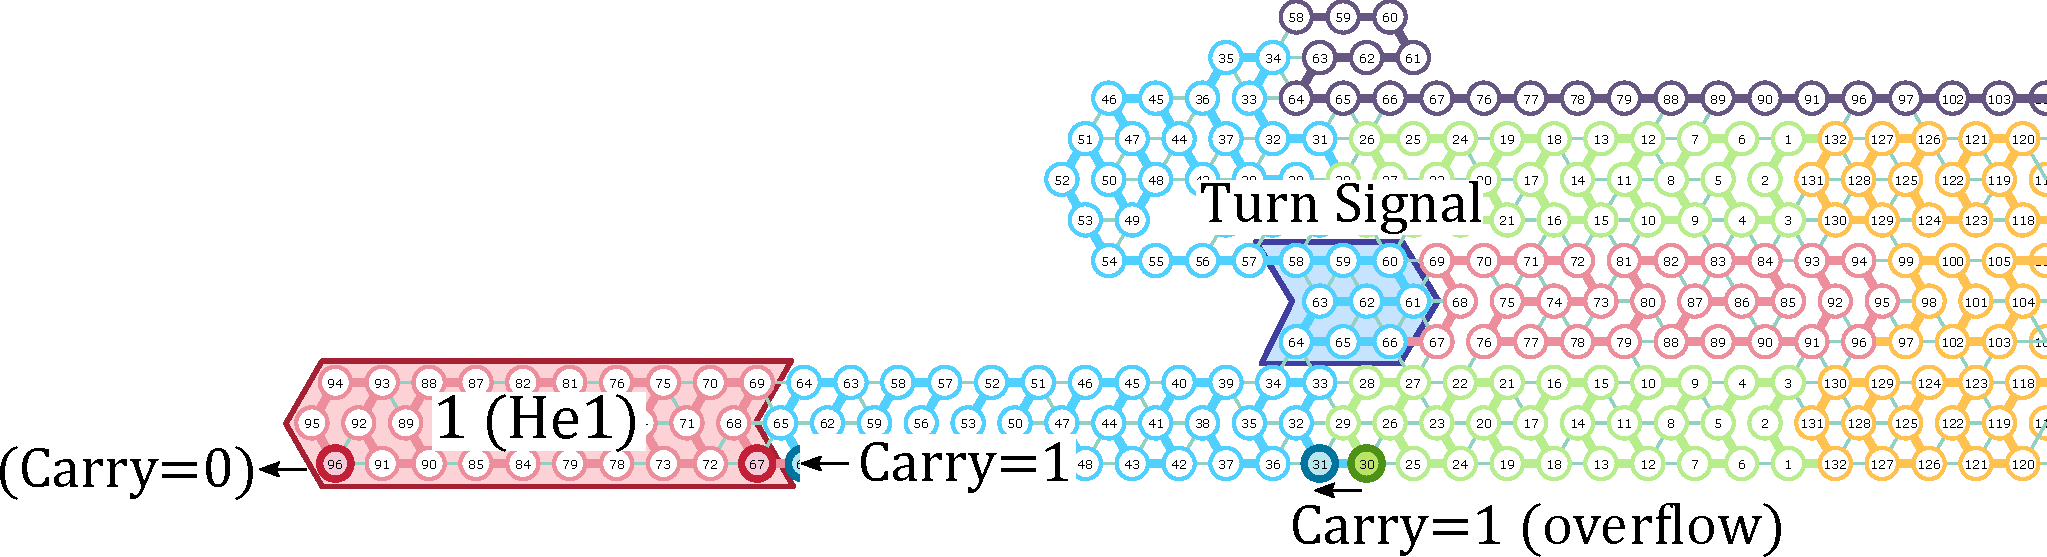
\includegraphics[width=\linewidth]{fig/svg/CounterEx15_2.pdf}
\end{minipage}
\end{tabular}

\caption{
(Left) Starting from the bottom, the Turn Signal above is too far for this L to fold into \texttt{Lcrn}.
It rather folds into \texttt{Lbe} and initiates bit expansion.
(Right) Without anything around, the succeeding H folds into a glider (brick \texttt{He1}).
}
\label{fig:overflowex2-3}
\end{figure}


\begin{figure}[tb]
\centering
\begin{tabular}{c}
 \begin{minipage}{0.45\linewidth}
 
\centering
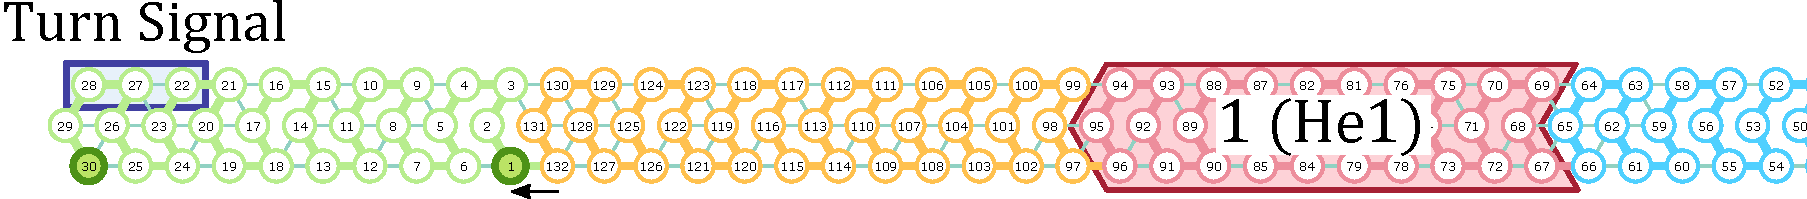
\includegraphics[width=\linewidth]{fig/svg/CounterEx17_3.pdf}

\end{minipage}
\begin{minipage}{0.05\linewidth}
\centering
{\large $\Rightarrow$}
\end{minipage}
 \begin{minipage}{0.5\linewidth}

\centering
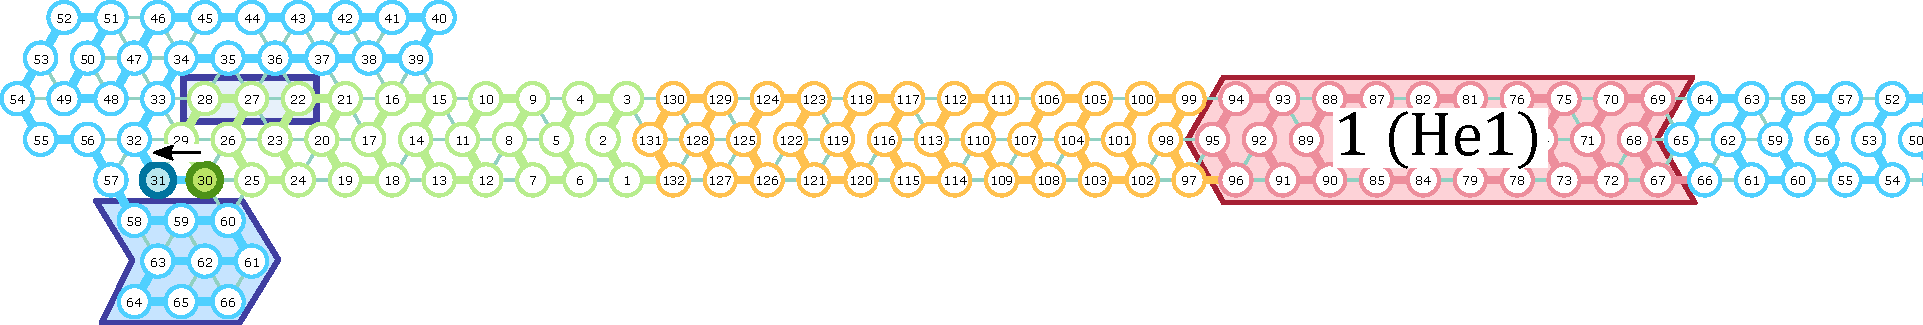
\includegraphics[width=\linewidth]{fig/svg/CounterEx18_2.pdf}

\end{minipage}
\end{tabular}

\caption{
The succeeding R and F also fold into respective glider-like bricks.
(Left) This brick of F (\texttt{Fnb}) exposes Turn Signal \texttt{28}{-}\texttt{27}{-}\texttt{22} (boxed), which is usually ``hidden" under the previous zag.
(Right) The exposed \texttt{28}{-}\texttt{27}{-}\texttt{22} (boxed) triggers the folding of next L into a special brick (\texttt{Lcre}) for left carriage-return.
}
\label{fig:overflowex4}
\end{figure}

%%%%%%%%%%%%
%\begin{figure}[h]
%\centering
%
%	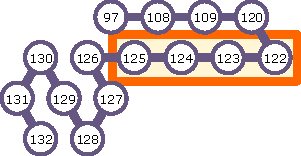
\includegraphics[width=5cm]{fig/svg/zeroBit01.pdf}
%
%\caption{0ビットからカウントを始める場合のシード。モジュールR用のターンシグナル部分とキャリーを与える部分が含まれている。}
%\label{fig:0bit_01}
%\end{figure}
%\begin{figure}[h]
%\centering
%
%	\includegraphics[width=5cm]{fig/svg/zeroBit02.pdf}
%
%\caption{モジュールFが自立する構造(グライダー)に折りたたまれジグ方向へ進む。}
%\label{fig:0bit_02}
%\end{figure}
%\begin{figure}[h]
%\centering
%
%	\includegraphics[width=5cm]{fig/svg/zeroBit03.pdf}
%
%\caption{モジュールLがFのターンシグナルと結合して左ターンする。}
%\label{fig:0bit_03}
%\end{figure}
%\begin{figure}[h]
%\label{fig:0bit_04}\centering
%
%	\includegraphics[width=5cm]{fig/svg/zeroBit04.pdf}
%
%\caption{モジュールHがザグ方向へ進む。}
%\label{fig:0bit_04}
%\end{figure}
%\begin{figure}[h]
%\centering
%
%	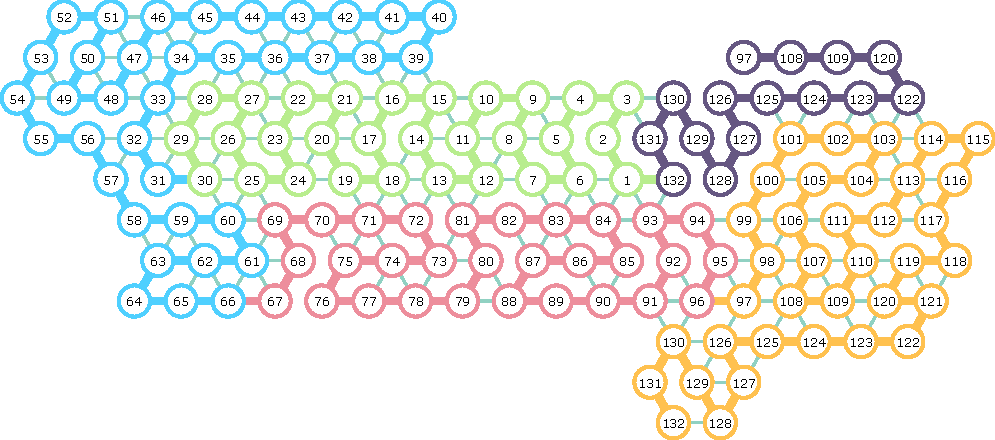
\includegraphics[width=5cm]{fig/svg/zeroBit05.pdf}
%
%\caption{モジュールRがシードのターンシグナルと結合して右ターンし通常のカウントが開始される。}
%\label{fig:0bit_05}
%\end{figure}
%
%
%\subsection{0ビットからのカウントアップ}
%有限カウンタでは、1からカウントを始めたとしてもビット幅を定めるために、そのビット幅分の0が記述される。
%しかし、この無限カウンタではビット幅が拡張できるため0ビットからのカウントアップすなわち、カウントをの値をシードに記述せずにカウントアップを始めることができる。
%シードがカウントの値を持たないのであれば、右ターン用のターンシグナルさえあればいいため、図~\ref{fig:0bit_01}
%のようなシードから転写が始まる。
%転写が始まると、その上部には折りたたまれた構造が存在しないので、最初のモジュールFからオーバーフローした時と同じ振る舞いをする。
%モジュールFはグライダー形に折りたたまり、次のLはFと結合し左ターンする (図~\ref{fig:0bit_02}、\ref{fig:0bit_03})。
%ジグのモジュールFは下側に何も信号を出力しないため、この段階ではまだカウント値は0ビットである。
%次にザグに移り、モジュールH、右ターンをするRと続きジグへと移る (図~\ref{fig:0bit_04})。
%このジグで再びオーバーフローが起こり、ここではカウント値のビット幅が拡張され、値「1」のカウントが行われ、これまで通りのカウントが続く。


%\subsection{実装したoritatami system}
%今回実装した無限バイナリカウンタのoritatami systemは以下の通りである。なおルールセット$R$は表~\ref{table:rule}のように、シード$\sigma$は0ビットからカウントアップを始めるのであれば図~\ref{fig:0bit_01}のようになる。
%
%\begin{eqnarray*}
%\Sigma &=& \{ 1,2, \ldots , 132\}\\
%\delta &=& 3\\
%\alpha &=& 5\\
%w &=& p^\omega \quad (p= 1.2.....132)
%\end{eqnarray*}
%
%
%%%%%%%%%%%
%ルールセット一覧%
%%%%%%%%%%%
%
\tablecaption{Rule set}
\begin{center}
\begin{supertabular}[tb]{l l l l l}
\label{table:rule}
(1,6),&(13,72),&(29,32), &(65,68),&(88,93),\\
(1,74),&(13,81),&(29,33),&(65,69),&(89,93),\\
(1,75),&(14,18),&(29,40),&(65,84),&(91,130),\\
(1,77),&(14,29),&(29,60),&(67,131),&(91,96),\\
(1,80),&(14,30),&(29,69),&(67,72),&(92,96),\\
(1,81),&(15,28),&(30,32),&(67,84),&(93,130),\\
(1,84),&(15,39),&(30,33),&(67,88),&(93,132),\\
(1,93),&(15,72),&(30,39),&(68,72),&(94,99),\\
(2,21),&(15,76),&(30,40),&(68,83),&(95,97),\\
(3,130),&(15,81),&(30,60),&(68,84),&(95,98),\\
(3,131),&(15,90),&(31,36),&(68,87),&(96,130),\\
(3,64),&(15,91),&(31,65),&(69,130),&(96,132),\\
(3,65),&(16,21),&(32,35),&(69,131),&(97,102),\\
(3,84),&(16,27),&(32,36),&(70,75),&(97,108),\\
(3,91),&(16,38),&(32,37),&(70,81),&(97,126),\\
(3,93),&(16,39),&(32,38),&(70,87),&(98,102),\\
(3,95),&(16,71),&(32,56),&(71,74),&(98,106),\\
(4,21),&(16,72),&(32,57),&(71,75),&(98,107),\\
(4,83),&(17,20),&(33,35),&(71,81),&(98,108),\\
(4,84),&(17,21),&(33,47),&(71,86),&(99,106),\\
(4,9),&(17,26),&(33,48),&(71,87),&(99,127),\\
(5,20),&(17,27),&(33,61),&(72,79),&(99,129),\\
(5,8),&(17,70),&(33,63),&(72,80),&(100,105),\\
(5,85),&(17,88),&(33,64),&(73,78),&(101,104),\\
(5,9),&(18,25),&(34,39),&(73,80),&(101,124),\\
(5,90),&(18,27),&(34,45),&(73,81),&(101,125),\\
(5,91),&(18,67),&(34,46),&(73,84),&(102,123),\\
(6,15),&(18,69),&(34,47),&(73,88),&(103,108),\\
(6,19),&(18,70),&(34,58),&(74,77),&(103,113),\\
(6,81),&(18,71),&(34,63),&(74,78),&(103,114),\\
(6,82),&(18,72),&(34,64),&(74,83),&(103,122),\\
(6,83),&(18,88),&(35,39),&(74,84),&(103,123),\\
(6,84),&(19,24),&(36,43),&(74,87),&(104,107),\\
(6,91),&(19,26),&(36,44),&(75,132),&(104,108),\\
(6,92),&(19,71),&(36,45),&(75,83),&(104,113),\\
(7,12),&(19,81),&(36,60),&(75,96),&(104,115),\\
(7,13),&(20,23),&(36,64),&(76,81),&(106,111),\\
(7,18),&(20,24),&(37,42),&(76,87),&(107,109),\\
(7,83),&(21,37),&(37,43),&(76,93),&(107,110),\\
(7,89),&(22,27),&(38,41),&(76,95),&(108,124),\\
(8,11),&(22,28),&(38,42),&(77,80),&(108,125),\\
(8,12),&(22,36),&(38,43),&(77,81),&(109,114),\\
(8,18),&(22,75),&(40,45),&(77,86),&(109,120),\\
(8,73),&(22,76),&(40,58),&(77,87),&(109,123),\\
(8,78),&(22,78),&(41,43),&(77,92),&(110,113),\\
(8,87),&(23,26),&(41,44),&(77,93),&(110,114),\\
(9,17),&(23,27),&(41,45),&(78,127),&(110,119),\\
(9,72),&(23,28),&(41,57),&(78,132),&(110,120),\\
(9,73),&(23,73),&(42,54),&(78,99),&(111,117),\\
(9,83),&(23,74),&(42,56),&(79,84),&(112,117),\\
(9,86),&(23,75),&(43,48),&(79,88),&(113,116),\\
(9,87),&(24,71),&(44,47),&(79,90),&(113,117),\\
(10,15),&(24,72),&(44,48),&(79,96),&(114,122),\\
(10,67),&(25,30),&(45,51),&(79,97),&(115,120),\\
(10,79),&(25,60),&(46,51),&(79,98),&(116,120),\\
(10,81),&(25,69),&(47,49),&(80,83),&(118,121),\\
(10,85),&(25,73),&(47,50),&(80,84),&(118,123),\\
(11,14),&(26,29),&(47,51),&(80,88),&(119,121),\\
(11,15),&(26,30),&(48,50),&(80,89),&(119,122),\\
(11,64),&(26,31),&(49,53),&(80,95),&(119,123),\\
(11,66),&(26,65),&(49,54),&(80,96),&(120,123),\\
(11,78),&(26,66),&(52,57),&(81,132),&(121,126),\\
(12,33),&(26,69),&(55,60),&(81,89),&(122,126),\\
(12,61),&(26,70),&(58,63),&(81,96),&(124,129),\\
(12,63),&(26,71),&(59,62),&(82,87),&(125,127),\\
(12,64),&(26,72),&(59,63),&(82,93),&(125,128),\\
(12,65),&(27,35),&(60,66),&(82,94),&(125,129),\\
(12,66),&(27,36),&(60,69),&(82,95),&(126,129),\\
(12,77),&(27,64),&(61,66),&(83,86),&(126,130),\\
(12,78),&(27,66),&(61,67),&(83,87),&(127,129),\\
(12,81),&(27,67),&(61,68),&(83,92),&(127,132),\\
(12,88),&(27,68),&(61,69),&(83,93),&(128,130),\\
(13,18),&(27,69),&(62,65),&(84,131),&(128,131),\\
(13,30),&(28,33),&(62,66),&(84,93),&(128,132)  \\
(13,31),&(28,35),&(64,69),&(85,130),&\\
(13,32),&(28,60),&(64,85),&(85,90),&\\
(13,33),&(29,31),&(65,67),&(86,90),&\\
\end{supertabular}
\end{center}



\section{Conclusion}
In this work, we have implemented an infinite binary counter in oritatami system by improving the existing binary counter in order to handle an overflow.
We divide the transcript of the infinite binary counter into four modules.
The counter is folded into zig-zag manner and both of zig and zag have $4n{-}3$ modules in order for module L and module R to left turn and to right turn, respectively.
The transcript of the existing finite counter has to bind to other modules, on the other hand, our transcript of the infinite counter can fold into a module by inner bounds.

%チューリング完全なシステムより少ないビードタイプで実装した
%Heighway dragon への応用も考えられる


\begin{acknowledgements}
This work is supported in part by KAKENHI Grant-in-Aid for Challenging Research (Exploratory) No.~18K19779 and JST Program to Disseminate Tenure Tracking System No.~6F36, both granted to S.~S.
\end{acknowledgements}


%%%%%%%%%%%%%%%%%
%In this paper, we have improved the existing finite binary counter by equipping it with a function of bit expansion at an overflow.
%Applications of our infinite counter include simulation of countably many Turing-machines in parallel for proving the undecidability of various properties of oritatami system, and folding of fractals.
%For their sake, this counter should be optimized, for example, by reducing bead types, shortening the period, or simplifying its rule set, though such optimization problems are computationally hard in general \cite{RulesetOptimization,OtaS2017}.


%\centering
%\begin{table}[tb]
%\begin{tabular}{c c c c}
%\begin{minipage}{25mm}
%	\centering
%       \scalebox{0.5}{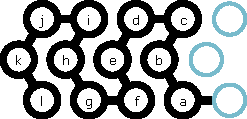
\includegraphics{fig/svg/bglider.pdf}}
%\end{minipage} &
%\begin{minipage}{25mm}
%	\centering
%       \scalebox{0.5}{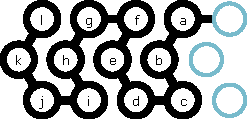
\includegraphics{fig/svg/tglider.pdf}}
%\end{minipage} &
%\begin{minipage}{30mm}
%	\centering
%       \scalebox{0.5}{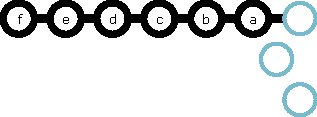
\includegraphics{fig/svg/plane.pdf}}
%\end{minipage} &
%\begin{minipage}{25mm}
%	\centering
%       \scalebox{0.5}{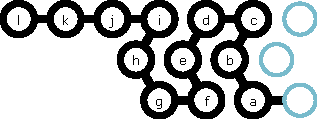
\includegraphics{fig/svg/spiral.pdf}}
%\end{minipage}\\
%
%\begin{minipage}{25mm}
%	\centering
%       \scalebox{0.5}{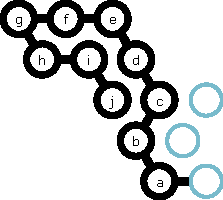
\includegraphics{fig/svg/horn.pdf}}
%\end{minipage} &
%\begin{minipage}{30mm}
%	\centering
%       \scalebox{0.5}{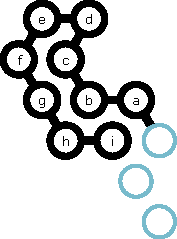
\includegraphics{fig/svg/kar.pdf}}
%\end{minipage} &
%\begin{minipage}{25mm}
%	\centering
%       \scalebox{0.5}{\includegraphics{fig/svg/roof.pdf}}
%\end{minipage}\\
%
%\begin{minipage}{25mm}
%	\centering
%       \scalebox{0.5}{\includegraphics{fig/svg/fault.pdf}}
%\end{minipage} &
%\begin{minipage}{30mm}
%	\centering
%       \scalebox{0.5}{\includegraphics{fig/svg/cliff.pdf}}
%\end{minipage}\\
%
%\end{tabular}
%\end{table}



\bibliographystyle{splncs03}
\bibliography{nc2020}

%\begin{thebibliography}{1}
%
%\bibitem{AdChGoHu2001}
%Leonard Adleman, Qi Chang, Ashish Goel, and Ming-Deh Huang, 
%Running time and program size for self-assembled squares, 
%In Proc. STOC 2001, ACM, 740-748, 2001. 
%
%\bibitem{BrChDoKaSe2013}
%Nathaniel Bryans, Ehsan Chiniforooshan, David Doty, Lila Kari, and Shinnosuke Seki, 
%The power of nondeterminism in self-assembly, 
%\textit{Theory of Computing}, vol. 9, 1-29, 2013.
%
%\bibitem{EvansPhD}
%Constantine Glen Evans, 
%Crystals that Count! Physical Principles and Experimental Investigations of {DNA} Tile Self-Assembly, 
%Ph.D. thesis, Caltech, 2014.
%
%\bibitem{GeMeScSe2019}
%Cody Geary, Pierre-\'{E}tienne Meunier, Nicolas Schabanel, and Shinnosuke Seki, 
%Oritatami: A computational model for molecular co-transcriptional folding, 
%\textit{International Journal of Molecular Sciences} vol. 20(9), 2259, 2019. Its conference version was published in Proc. MFCS 2016. 
%
%\bibitem{GearyRothemundAndersen2014}
%Cody Geary, Paul W. K. Rothemund, and Ebbe S. Andersen, 
%A single-stranded architecture for cotranscriptional folding of {RNA} nanostructures, 
%\textit{Science} vol 345(6198), 799-804, 2014.
%
%\bibitem{MasudaSekiUbukata2018}
%Yusei Masuda, Shinnosuke Seki, and Yuki Ubukata, 
%Towards the algorithmic molecular self-assembly of fractals by cotranscriptional folding, 
%In Proc. CIAA 2018, LNCS 10977, Springer, 261-273, 2018.
%
%\bibitem{McClung2006} 
%C. Robertson McClung, 
%Plant circadian rhythms, 
%\textit{The Plant Cell}, vol. 18, 792-803, 2006.
%
%\bibitem{Minsky1967}
%Marvin Minsky, 
%Computation: Finite and Infinite Machines, 
%Prentice-Hall, Inc., 1967. 
%
%\bibitem{RothemundWinfree2000}
%Paul W. K. Rothemund and Erik Winfree, 
%The program-size complexity of self-assembled squares (extended abstract), 
%In Proc. STOC 2000, ACM, 459-468, 2000.
%
%\bibitem{WinfreePhD}
%Erik Winfree, 
%Algorithmic Self-Assembly of {DNA}, 
%Ph.D. thesis, Caltech, 1998.
%
%\bibitem{GeMeScSe2018}
%Cody Geary and Pierre-\'Etienne Meunier and Nicolas Schabanel and Shinonsuke Seki,
%Proving the {T}uring Universality of Oritatami Cotranscriptional Folding,
%Proc. ISAAC 2018,
%23:1 -- 23:13,2018.
%
%
%\end{thebibliography}
  
\end{document}
